\documentclass[preprint,12pt]{elsarticle}
\usepackage[T1]{fontenc}
\usepackage{algpseudocode}
\usepackage{lmodern}
\usepackage{amsmath,amssymb,amsthm,graphicx}
\usepackage{float}
\newtheorem{remark}{Remark}
\usepackage[section]{placeins}
\floatstyle{ruled}
\newfloat{algorithm}{tbp}{loa}
\usepackage{enumitem}
\floatname{algorithm}{Algorithm}
\usepackage{tikz}
\usetikzlibrary{arrows.meta}
\usepackage[hidelinks,hypertexnames=false]{hyperref}
\hypersetup{pdfauthor={Chaoyang Li, Xiaohan Li, Zhaowen Li}}
\journal{Applied Soft Computing}
\newtheorem{definition}{Definition}
\newtheorem{proposition}{Proposition}
\numberwithin{equation}{section}
\emergencystretch=2em
\begin{document}
\begin{frontmatter}
\title{Prediction-Constrained Cost-Sensitive Attribute Reduction for Label Distribution Learning via Directed Granular-Ball Computing}
% Elsevier elsarticle frontmatter; place after title and before abstract.
\author[aff1]{Chaoyang Li}
\ead{lichaoyang1@gdust.edu.cn}
\author[aff2]{Xiaohan Li}
\ead{xiaohanl06@student.must.edu.mo}
\author[aff3]{Zhaowen Li\corref{cor1}}
\ead{lzwli@ptu.edu.cn}
\cortext[cor1]{Corresponding author.}
\affiliation[aff1]{organization={Guangdong University of Science and Technology},
  city={Dongguan}, postcode={523083}, state={Guangdong}, country={China}}
\affiliation[aff2]{organization={Faculty of Innovation Engineering, Macau University of Science and Technology},
  city={Macau}, country={China}}
\affiliation[aff3]{organization={Fujian Key Laboratory of Financial Information Processing, Putian University},
  city={Putian}, postcode={351100}, state={Fujian}, country={China}}

\begin{abstract}
Existing attribute reduction methods for Label Distribution Learning (LDL) often overlook the substantial variation in attribute acquisition costs, failing to balance prediction performance against real-world resource constraints. To address this, we propose a cost-constrained attribute reduction framework for LDL that explicitly incorporates attribute acquisition costs while retaining distributional supervision. We introduce a local distribution-information weight coupled with a source-dependent directed dissimilarity metric to capture both supervised association and intrinsic geometric structures. Based on this, a deterministic granular-ball model is constructed, equipped with a non-monotone granular dependency derived from normalized training representation error. To handle non-monotonicity, we formulate attribute reduction as a minimum-cost subset selection problem subject to an internal prediction-loss constraint, solved via a hybrid approach comprising a constructive heuristic, an exact backtracking algorithm, and an exchange refinement step. Extensive evaluations across twenty-five native LDL benchmark datasets—utilizing reserved audit partitions, matched-cost label-free controls, and common-budget ablations—demonstrate that our framework reduces acquisition costs by over two orders of magnitude (e.g., from 1,648 to ~10 on Natural Scene, and from 2,841 to ~19 on fbp5500) without sacrificing prediction accuracy. Benchmark comparisons against five published scoring cores spanning 2022–2025 confirm that published selectors incur two to five times higher costs for comparable or inferior predictive performance. Furthermore, our analysis identifies a near-degenerate regime—prevalent on twenty of the twenty-five benchmarks—where zero-cost configurations are optimal, and a predictor-sensitivity study shows that the feasibility guard tracks the deployed predictor: substituting a ridge predictor revives nine degenerate benchmarks, on six of which the selected low-cost subsets (1--6\% of full-set cost) outperform both the zero-cost and full-cost references. These results emphasize the necessity of feasibility guarantees over conventional lossless reduction.
\end{abstract}
\begin{keyword}
Label distribution learning \sep Attribute reduction \sep Attribute acquisition cost \sep Granular computing \sep Directed dissimilarity
\end{keyword}
\end{frontmatter}
% Consolidated manuscript draft. Experimental evidence remains developmental.
\section{Introduction}
\label{sec:introduction}
\subsection{Research background and related work}
Label distribution learning (LDL) represents each instance by a vector of non-negative description degrees summing to one~\cite{G1}. Unlike conventional multi-label annotations that merely indicate label presence or absence, LDL preserves rich quantitative information regarding the relative importance of different labels. LDL has demonstrated success across diverse domains, including crowd counting, facial expression recognition, and physiological prediction~\cite{ZW1,LS,QH}. However, converting native distributions into dominant labels or binary relevance sets inevitably loses fine-grained distributional information. Effective attribute reduction for LDL must therefore directly evaluate and respect the underlying distribution.

High-dimensional attribute spaces frequently contain redundant or uninformative features. While selecting an optimal feature subset enhances model interpretability and lowers measurement overhead, reducing attribute cardinality does not inherently guarantee improved predictive performance. Furthermore, simple cardinality metrics fail to account for deployment costs when individual attributes carry different acquisition burdens. Cost-sensitive learning addresses various operational expenses, such as test cost, misclassification cost, and computational or human resources~\cite{Turney2000}; for example, cost-sensitive embedded feature selection has been explored within support vector machines~\cite{AL}. In rough set theory, test-cost-sensitive reduction seeks optimal attribute subsets under explicit budget constraints: Min et al.~\cite{Min2014TestCost} formulated cost-constrained selection as a constraint satisfaction problem solved via backtracking heuristics, whereas decision-theoretic rough sets model attribute reliance using decision costs~\cite{Jia2013MinCost}. Although these studies share our concept of acquisition cost, they fundamentally rely on discrete decision classes. Existing LDL feature selectors—including granular and neighborhood models—typically score attributes based on information metrics and apply cardinality or threshold cuts. To the best of our knowledge, none formulate the task as finding a \emph{minimum-acquisition-cost subset subject to an explicit prediction-loss constraint}. This formulation shifts the conventional paradigm: rather than minimizing prediction loss for a fixed subset size, we minimize total acquisition cost while guaranteeing that a designated predictor's internal training loss remains within the full-attribute reference baseline. This directly addresses a critical deployment challenge: identifying the cheapest set of measurements that provably maintains predictive feasibility. Here, test cost specifically refers to the expense of acquiring attribute values for new instances during prediction, distinct from the offline execution time of the reduction algorithm itself.

Rough sets and neighborhood models offer a rigorous foundation for evaluating attribute-dependent information structures~\cite{CARS,NRS}. Extending these models to LDL requires adapting the supervisory signal from crisp classes to continuous distributions. Qian et al.~\cite{QX} incorporated feature similarity alongside label correlation, Deng et al.~\cite{DL} proposed a dual-similarity neighborhood fuzzy entropy spanning both attribute and label spaces, and Qian et al.~\cite{QD} handled incomplete distributions via neighborhood-tolerance discrimination. Recent extensions further enrich this lineage: Lin et al.~\cite{LW} integrated sparse regularization, label correlation, and mutual information into feature weighting; Shu et al.~\cite{Shu2024Specific} jointly modeled common and label-specific features; Deng et al.~\cite{Deng2025LDNF} formulated neighborhood fuzzy rough sets for LDL; Zhao et al.~\cite{Zhao2026IWNRS} developed an information-weighted neighborhood model with a conditional discrimination index; and Chen et al.~\cite{Chen2025OnlineLDL} explored online selection driven by label importance and correlation. Additionally, information-theoretic measures—such as mutual information, fuzzy entropy~\cite{QHM,WH2,XQ}, neighborhood self-information~\cite{WH1,XJ,JZ}, and hierarchical variants~\cite{LH}—evaluate feature utility based on distributional information content. While these methods explore diverse representations and search strategies, their existence underscores the need to define precisely what an acquisition-cost-aware granular framework adds to the field.

A closely related domain is feature reduction for multi-label learning, as surveyed by Kashef et al.~\cite{KP}. Representative approaches include ReliefF-based multi-label weighting~\cite{RM1}, multivariate mutual-information filters~\cite{LK}, and fuzzy relative discernibility ranking~\cite{QX2}. Although multi-label techniques handle label correlations, they ultimately target binary relevance structures and remain unequipped for full description-degree distributions. Similarly, metaheuristic attribute reduction algorithms—spanning evolutionary, swarm, and local search strategies~\cite{HX,NG,ZS,AE,OM}—optimize classical dependency or information criteria. Such search mechanisms are orthogonal to our primary contribution and could, in principle, complement or substitute the constructive search employed here.

Granular-ball computing has also emerged as a powerful paradigm in LDL feature selection. Qian et al.~\cite{Qian2023GBLDL} developed a granular-ball fuzzy rough set incorporating distributional similarity and local consistency. Granular generation itself remains a pivotal design choice: GBG++ provides fast and stable generation for classification~\cite{Xie2024GBG}, efficient adaptive generation methods continue to evolve~\cite{Xia2023GBadaptive}, and unified granular-ball models connect Pawlak and neighborhood rough sets within a common theoretical framework~\cite{Xia2023GBRS}. The present work builds upon this granular foundation by introducing a source-dependent information geometry, a deterministic distribution-driven ball construction, and an explicit acquisition-cost objective. Rather than merely applying granular balls to LDL, our motivation lies in formalizing the mathematical and empirical interplay between supervised geometry, regenerated granules, and prediction-feasible cost minimization.

\subsection{Motivation and contributions}
Three interconnected challenges motivate the proposed framework. First, the informative value of an attribute varies across individual objects. When the local mean label distribution within an attribute-induced neighborhood deviates from the global label distribution, that attribute exhibits local distributional discrimination. We quantify this association using a regularized divergence weight. Because this weight depends intrinsically on the source object, the resulting dissimilarity measure is directed. Additionally, a raw geometric term preserves subtle distinctions made by non-constant attributes that carry zero information weight. Critically, this distributional association serves as an exploratory selection signal rather than a strict guarantee of downstream predictive performance.

Second, altering the attribute subset dynamically reshapes the granular topology. Although the directed dissimilarity exhibits monotonicity under attribute inclusion when dataset statistics and normalization parameters remain fixed, regenerated granular balls are not necessarily nested. Consequently, granular dependency does not monotonically increase with attribute inclusion. Mistaking distance monotonicity for a dependency theorem leads to unsound pruning and stopping heuristics. To address this, our framework explicitly accommodates signed dependency gains and defines the exact structural properties that hold under the training representation.

Third, granular representation quality and predictor validation loss assess fundamentally different metrics. A subset yielding a superior training representation does not inherently generalize better to unseen label distributions. We therefore formulate attribute reduction as minimizing additive acquisition costs subject to an explicit, training-internal prediction-loss constraint. Granular dependency guides the constructive search trajectory, while the target predictor's internal loss enforces feasibility. Figure~\ref{fig:intro-roles} illustrates this functional separation, which retains the structural benefits of granular computing without relying on unjustified predictive guarantees derived purely from dependency metrics.

\begin{figure}[htbp]
	\centering
	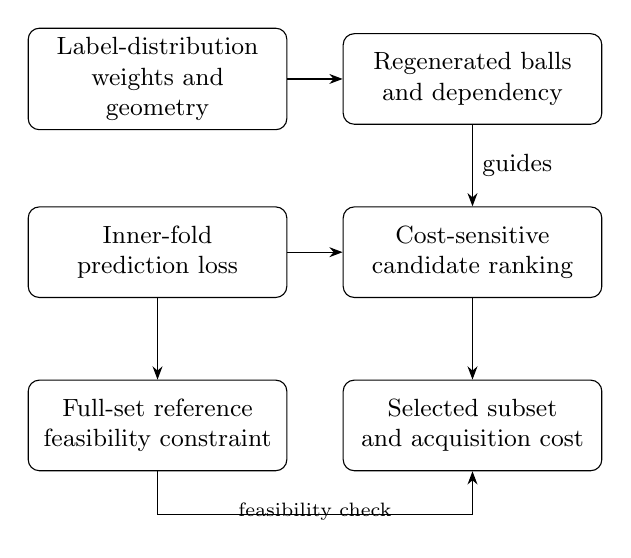
\begin{tikzpicture}[>=Stealth, every node/.style={font=\small}, box/.style={draw,rounded corners,align=center,text width=3.05cm,minimum height=1.15cm}]
		\node[box] (w) at (0,0) {Label-distribution\\weights and geometry};
		\node[box] (g) at (4,0) {Regenerated balls\\and dependency};
		\node[box] (h) at (4,-2.2) {Cost-sensitive\\candidate ranking};
		\node[box] (l) at (0,-2.2) {Inner-fold\\prediction loss};
		\node[box] (f) at (0,-4.4) {Full-set reference\\feasibility constraint};
		\node[box] (o) at (4,-4.4) {Selected subset\\and acquisition cost};
		\draw[->] (w)--(g);
		\draw[->] (g)--node[right]{guides}(h);
		\draw[->] (l)--(h);
		\draw[->] (l)--(f);
		\draw[->] (h)--(o);
		\draw[->] (f.south)--++(0,-0.55)-| (o.south);
		\node[font=\scriptsize] at (2,-5.5) {feasibility check};
	\end{tikzpicture}
	\caption{Decoupled roles of granular information and predictive feasibility. The schematic depicts information flow during attribute selection; internal constraint satisfaction does not guarantee loss preservation on held-out test sets.}
	\label{fig:intro-roles}
\end{figure}

The principal contributions of this work are summarized as follows:
\begin{enumerate}
	\item \textbf{LDL-Driven Directed Dissimilarity:} We construct a local information weight tailored to label distributions and combine it with raw attribute geometry to formulate a source-dependent directed dissimilarity. We prove its boundedness and fixed-statistics attribute monotonicity without requiring metric axioms or asserting monotonicity for regenerated granular dependency.
	\item \textbf{Deterministic Granular Dependency Framework:} We introduce distribution consistency and eligible-ball dependency within a deterministic granular ball construction. Through a within--between error decomposition, we show that dependency measures normalized training representation error reduction (using global-distribution fallback for ineligible objects), where signed dependency gains naturally capture structural variations under feature addition.
	\item \textbf{Constrained Acquisition-Cost Optimization:} We formalize minimum-acquisition-cost reduction under an internal prediction-loss constraint, proposing both a dependency-guided heuristic search and an exact backtracking reference algorithm. We establish the finite feasible termination of the heuristic and the global cost optimality of the completed exact search. Furthermore, an optional local deletion/exchange post-processing phase is designed to strictly lower cost while maintaining feasibility.
	\item \textbf{Rigorous Empirical Benchmarking:} We evaluate our framework across twenty-five native LDL benchmarks using repeated training partitions, reserved audit labels, matched-cost label-free controls, and budget-matched ablations, against five published scoring cores spanning 2022--2025. Results demonstrate that our method reduces acquisition cost by over two orders of magnitude (e.g., from $1648$ to approximately $10$ on the Natural Scene dataset) while consistently outperforming label-free baselines of equivalent cost. A guard ablation shows that conventional guard-free selection spends acquisition budget for predictions worse than the free default on the degenerate domains, and a predictor-sensitivity study shows the guard certifying informative low-cost subsets (dominating both zero-cost and full-cost references on six of nine revived datasets) once a suitable predictor is deployed.
\end{enumerate}

In summary, the proposed methodology integrates distribution-aware granular information with explicit predictive feasibility constraints. Its theoretical bounds apply strictly to the defined representation and search mechanisms, whereas its predictive efficacy is validated empirically across specified learners, cost structures, and data splits. Ultimately, the framework delivers a cost-efficient attribute subset guaranteed to satisfy internal predictive feasibility; where a simple mean-distribution predictor already matches the full-attribute baseline, the method correctly identifies and returns an empty subset at zero cost, and when a stronger predictor makes a domain informative again, it certifies low-cost subsets that dominate wholesale acquisition.

\section{Preliminaries}
% Proposed LDL foundations, 2026-09-30.
% This replaces the crisp-decision-system setup only.
% No claim about adaptive granular-ball dependency monotonicity is made.
\subsection{Test-cost-sensitive label distribution decision information system}
\label{subsec:ldl-system}

Let $O=\{o_1,\dots,o_n\}$ be a finite, non-empty set of objects, $A=\{a_1,\dots,a_m\}$ a finite, non-empty set of conditional attributes, and $\mathcal{Y}=\{y_1,\dots,y_q\}$ a finite, non-empty set of labels. Each attribute $a\in A$ induces a mapping $a: O \to V_a$, where $V_a$ denotes the domain of attribute $a$. To handle hybrid feature spaces, we partition $A$ as
\[
A = A_n \cup A_c, \qquad A_n \cap A_c = \varnothing,
\]
where $A_n$ and $A_c$ designate numerical and categorical attribute subsets, respectively. Either subset may be empty.

\begin{definition}[Label Distribution Decision Information System]
	\label{def:ldl-system}
	A label distribution decision information system is a tuple
	\[
	\mathcal{S}_L = (O, A, \mathcal{Y}, L),
	\]
	where $L = (\ell_i^k)_{n\times q}$ is the label distribution matrix satisfying the simplex constraints:
	\begin{equation}
		\ell_i^k \in [0,1], \qquad \sum_{k=1}^q \ell_i^k = 1 \quad (i=1,\dots,n;\ k=1,\dots,q).
		\label{eq:label-simplex}
	\end{equation}
	The label distribution associated with object $o_i$ is represented by the vector
	\begin{equation}
		\boldsymbol{\ell}(o_i) = (\ell_i^1, \dots, \ell_i^q),
		\label{eq:label-vector}
	\end{equation}
	where $\ell_i^k$ quantifies the description degree of label $y_k$ for object $o_i$~\cite{G1}.
\end{definition}

In our framework, the complete distribution vector $\boldsymbol{\ell}(o_i)$ serves directly as the supervisory decision signal. Rather than collapsing the vector to the most dominant label, this formulation explicitly retains fine-grained relative importances. Importantly, description degrees reflect quantitative supervisory weights rather than posterior class probabilities.

The proposed information system builds upon Pawlak's classical rough set model~\cite{CARS}, incorporating neighborhood-based extensions designed for hybrid data types~\cite{NRS,Y1,HY}. Whereas traditional attribute reduction techniques rely on heuristic searches guided by dependency or information measures over crisp equivalence classes~\cite{SZ,XW,YC,ZM}, our model fundamentally differs in two key respects: its decision representation is distributional, and its reduction objective explicitly incorporates attribute acquisition costs.

\begin{definition}[Soft Decision Representation]
	\label{def:soft-decision}
	For each label $y_k \in \mathcal{Y}$, define a fuzzy decision set $D_k$ on $O$ via the membership function
	\begin{equation}
		\mu_{D_k}(o_i) = \ell_i^k \quad (i=1,\dots,n;\ k=1,\dots,q).
		\label{eq:soft-decision}
	\end{equation}
	The collection $\mathcal{D}_L = \{D_1, \dots, D_q\}$ constitutes the soft decision representation induced by $L$.
\end{definition}

According to Eq.~\eqref{eq:label-simplex}, the membership functions satisfy
\begin{equation}
	\sum_{k=1}^q \mu_{D_k}(o_i) = 1 \quad \text{for all } o_i \in O.
	\label{eq:soft-partition}
\end{equation}
Consequently, $\mathcal{D}_L$ forms a fuzzy partition-of-unity over $O$. Unlike traditional decision tables, $\mathcal{D}_L$ does not induce mutually disjoint crisp equivalence classes; an object $o_i$ may simultaneously possess positive membership across multiple fuzzy decision sets $D_k$. Therefore, theoretical results relying on classical crisp partitions cannot be assumed directly and must be formally re-evaluated within this soft decision space.

For label-weighted statistics introduced in subsequent sections, the total description mass of label $y_k$ is defined as
\begin{equation}
	M_k = \sum_{i=1}^n \ell_i^k.
	\label{eq:label-mass}
\end{equation}
Any statistical quantity involving $M_k$ in the denominator is valid if and only if $M_k > 0$. A label with $M_k = 0$ carries zero description mass across all sample instances and is naturally excluded from label-weighted calculations.

\begin{definition}[Test-Cost-Sensitive System]
	\label{def:test-cost}
	A test-cost-sensitive label distribution decision information system is defined as
	\[
	\mathcal{S}_{L,c} = (O, A, \mathcal{Y}, L, c),
	\]
	where $c: A \to \mathbb{R}_{>0}$ assigns a positive acquisition cost to each attribute $a \in A$. Assuming additivity, the total cost of acquiring an attribute subset $P \subseteq A$ is
	\begin{equation}
		c(P) = \sum_{a \in P} c(a), \qquad \text{with } c(\varnothing) = 0.
		\label{eq:additive-cost}
	\end{equation}
\end{definition}

The strict positivity constraint $c(a) > 0$ ensures that the cost weighting term $c(a)^\lambda$ remains well-defined and bounded for any exponent $\lambda \le 0$. Furthermore, this condition guarantees strict monotonicity of acquisition costs under subset inclusion—that is, $c(P) < c(Q)$ whenever $P \subsetneq Q$—without imposing any structural monotonicity assumptions on the granular dependency function itself.

\begin{proposition}[Crisp Decision Representation as a Special Case]
	\label{prop:crisp-special-case}
	Suppose each row of $L$ is a one-hot vector (i.e., $\ell_i^k \in \{0, 1\}$ for all $i, k$). Define a discrete decision mapping $d: O \to \mathcal{Y}$ such that $d(o_i) = y_k$ if and only if $\ell_i^k = 1$. Then, each $D_k$ collapses to the indicator function of the crisp decision class
	\[
	C_k = \{o_i \in O : d(o_i) = y_k\}.
	\]
	Upon removing empty sets, $\{C_k\}$ forms a strict crisp partition of $O$.
\end{proposition}
\begin{proof}
	For any $o_i \in O$, there exists a unique index $k$ such that $\ell_i^k = 1$. Thus, $o_i$ belongs to exactly one decision class $C_k$, establishing that $\bigcup_{k=1}^q C_k = O$ and $C_k \cap C_h = \varnothing$ for all $k \neq h$. By Eq.~\eqref{eq:soft-decision}, the membership function reduces to
	\[
	\mu_{D_k}(o_i) = 
	\begin{cases}
		1, & \text{if } o_i \in C_k, \\
		0, & \text{if } o_i \notin C_k,
	\end{cases}
	\]
	which matches the indicator representation of the crisp set $C_k$.
\end{proof}

Proposition~\ref{prop:crisp-special-case} addresses the decision representation mapping exclusively. The theoretical reduction of approximation operators and dependency metrics to classical crisp rough set models remains a separate issue that must be established following their explicit definitions. No automatic transference of classical properties—such as monotonic dependency—is assumed.

\section{Label-distribution information and directed distance}

\subsection{Label-distribution-driven local relative information and directed dissimilarity}
\label{subsec:ldl-directed}

We retain the source-dependent, fixed-normalization directed aggregation structure, but introduce a unified information statistic applicable to both numerical and categorical attributes. This statistic quantifies the divergence between an attribute-induced local label profile and the global label profile. This modeling choice reflects a structured information-theoretic strategy rather than an empirical claim of absolute predictive optimality.

All statistical properties are evaluated on the fixed training object set $O$, remaining invariant when comparing alternative attribute subsets $P, Q \subseteq A$. Neither validation nor test labels are utilized during these computations.

\subsubsection{Global and attribute-induced local label profiles}
We define the global mean description degree for label $y_k$ across training instances as
\begin{equation}
	\bar{\ell}^k = \frac{1}{n} \sum_{i=1}^n \ell_i^k, \qquad \mathcal{K}_+ = \{k \in \{1,\dots,q\} : \bar{\ell}^k > 0\}.
	\label{eq:global-label-profile}
\end{equation}
The vector $\bar{\boldsymbol{\ell}} = (\bar{\ell}^1, \dots, \bar{\ell}^q)$ represents the global label distribution. By non-negativity constraint \eqref{eq:label-simplex}, $\bar{\ell}^k = 0$ implies $\ell_i^k = 0$ for all training instances $o_i \in O$. Such uninformative labels are naturally excluded from information ratios without altering non-zero description degrees.

For numerical attributes $a \in A_n$, training values are normalized to $[0, 1]$ via min-max scaling:
\begin{equation}
	z_a(o_i) = \begin{cases}
		\displaystyle\frac{a(o_i) - a_{\min}}{a_{\max} - a_{\min}}, & \text{if } a_{\max} > a_{\min}, \\[6pt]
		0, & \text{if } a_{\max} = a_{\min},
	\end{cases}
	\label{eq:numerical-normalization}
\end{equation}
where $a_{\min}$ and $a_{\max}$ denote the minimum and maximum values of attribute $a$ on $O$. Given a fixed kernel bandwidth $\tau_a > 0$, attribute-level pairwise affinities are defined as
\begin{equation}
	K_a(i,j) = \begin{cases}
		\displaystyle\exp\left( -\frac{(z_a(o_i) - z_a(o_j))^2}{2\tau_a^2} \right), & \text{if } a \in A_n, \\[8pt]
		1, & \text{if } a \in A_c \text{ and } a(o_i) = a(o_j), \\
		0, & \text{if } a \in A_c \text{ and } a(o_i) \neq a(o_j).
	\end{cases}
	\label{eq:attribute-affinity}
\end{equation}
For both feature modalities, the affinity matrix satisfies $0 \le K_a(i,j) \le 1$, $K_a(i,j) = K_a(j,i)$, and $K_a(i,i) = 1$.

We define the local support mass $s_a(i)$, the off-diagonal support mass $t_a(i)$, and the raw local label profile $\boldsymbol{u}_a(i)$ as follows:
\begin{align}
	s_a(i) &= \sum_{j=1}^n K_a(i,j), \qquad t_a(i) = \sum_{j \neq i} K_a(i,j) = s_a(i) - 1, \label{eq:local-support} \\
	u_a^k(i) &= \frac{\sum_{j=1}^n K_a(i,j) \ell_j^k}{s_a(i)}. \label{eq:raw-local-profile}
\end{align}
Note that $s_a(i) \ge 1$ and $t_a(i) \ge 0$, ensuring $\boldsymbol{u}_a(i) = (u_a^1(i), \dots, u_a^q(i))$ remains a valid label distribution. For categorical attributes, $\boldsymbol{u}_a(i)$ yields the conditional mean distribution for category $a(o_i)$; for numerical attributes, it computes a Gaussian kernel-weighted mean label profile around $z_a(o_i)$.

Because the raw profile includes the self-label $\boldsymbol{\ell}(o_i)$, small or sparse neighborhoods can introduce high variance. To stabilize local profile estimates, we incorporate a shrinkage hyperparameter $\beta > 0$ to construct a regularized local label profile:
\begin{align}
	\eta_a(i) &= \frac{t_a(i)}{t_a(i) + \beta}, \label{eq:profile-confidence} \\
	\widetilde{\boldsymbol{u}}_a(i) &= \eta_a(i) \boldsymbol{u}_a(i) + (1 - \eta_a(i)) \bar{\boldsymbol{\ell}}. \label{eq:regularized-local-profile}
\end{align}
The confidence factor $\eta_a(i)$ depends entirely on the supporting mass provided by other objects. If an object is completely isolated ($t_a(i) = 0$), $\eta_a(i) = 0$, causing the regularized profile to revert to the global profile $\bar{\boldsymbol{\ell}}$. This shrinkage mechanism balances local discrimination with sample support. Hyperparameters $\tau_a$ and $\beta$ are fixed strictly during training and are not re-tuned during feature subset evaluation.

\subsubsection{Normalized local relative information}
When the active label set satisfies $|\mathcal{K}_+| \ge 2$, we define the dataset-level information normalization factor
\begin{equation}
	B_L = \log_2 \left( \frac{1}{\min_{k \in \mathcal{K}_+} \bar{\ell}^k} \right) > 0.
	\label{eq:information-normalizer}
\end{equation}
The constant $B_L$ depends solely on the fixed global training label profile and remains independent of individual attributes or selected feature subsets.

\begin{definition}[Local Relative-Information Weight]
	\label{def:local-relative-weight}
	For $|\mathcal{K}_+| \ge 2$, the local relative-information weight of attribute $a$ at object $o_i$ is defined as
	\begin{equation}
		W_a(o_i) = \frac{1}{B_L} \sum_{k \in \mathcal{K}_+} \widetilde{u}_a^k(i) \log_2 \left( \frac{\widetilde{u}_a^k(i)}{\bar{\ell}^k} \right).
		\label{eq:relative-information-weight}
	\end{equation}
	If $|\mathcal{K}_+| = 1$, we set $W_a(o_i) = 0$ for all $a \in A$ and $o_i \in O$.
\end{definition}

The numerator in Eq.~\eqref{eq:relative-information-weight} measures the Kullback-Leibler (KL) divergence of the regularized local profile $\widetilde{\boldsymbol{u}}_a(i)$ from the global baseline $\bar{\boldsymbol{\ell}}$~\cite{SE}. Higher weight indicates that attribute $a$ creates a local neighborhood whose label dynamics deviate significantly from the dataset average, signaling strong local discrimination.

\begin{proposition}[Weight Bounds and Zero-Weight Conditions]
	\label{prop:relative-weight-bounds}
	For any attribute $a \in A$ and object $o_i \in O$, $0 \le W_a(o_i) \le 1$. Furthermore, when $|\mathcal{K}_+| \ge 2$:
	\[
	W_a(o_i) = 0 \quad \Longleftrightarrow \quad \widetilde{\boldsymbol{u}}_a(i) = \bar{\boldsymbol{\ell}}.
	\]
	Specifically, $W_a(o_i) = 0$ holds if $o_i$ lacks supporting neighbors ($t_a(i) = 0$), if $a$ is a constant attribute, or if all training instances share identical label distributions.
\end{proposition}
\begin{proof}
	Let $p_k = \bar{\ell}^k > 0$ and $r_k = \widetilde{u}_a^k(i)$ for $k \in \mathcal{K}_+$. By Gibbs' inequality (or log-sum inequality), $D_{\mathrm{KL}}(\boldsymbol{r} \parallel \boldsymbol{p}) \ge 0$, with equality holding if and only if $\boldsymbol{r} = \boldsymbol{p}$. For the upper bound,
	\[
	D_{\mathrm{KL}}(\boldsymbol{r} \parallel \boldsymbol{p}) = \sum_{k \in \mathcal{K}_+} r_k \log_2 r_k + \sum_{k \in \mathcal{K}_+} r_k \log_2 \left(\frac{1}{p_k}\right) \le 0 + \sum_{k \in \mathcal{K}_+} r_k B_L = B_L.
	\]
	Dividing by $B_L$ yields $0 \le W_a(o_i) \le 1$. If $t_a(i) = 0$, Eq.~\eqref{eq:regularized-local-profile} gives $\widetilde{\boldsymbol{u}}_a(i) = \bar{\boldsymbol{\ell}}$, implying $W_a(o_i) = 0$. For a constant attribute, $K_a(i,j) = 1$ for all $i,j$, which forces $\boldsymbol{u}_a(i) = \bar{\boldsymbol{\ell}}$ and thus $W_a(o_i) = 0$.
\end{proof}

\subsubsection{Hybrid discrepancy and directed aggregation}
To isolate the contribution of information weighting, we employ standard symmetric feature discrepancies. For a categorical attribute value $v \in V_a$, let
\begin{equation}
	r_a^k(v) = \frac{\sum_{i: a(o_i)=v} \ell_i^k}{|\{i : a(o_i)=v\}|}
	\label{eq:categorical-profile}
\end{equation}
denote the average description vector for value $v$. The hybrid discrepancy $\Delta_a(o_i, o_j)$ is defined as
\begin{equation}
	\Delta_a(o_i,o_j) = \begin{cases}
		|z_a(o_i) - z_a(o_j)|, & \text{if } a \in A_n, \\[4pt]
		\displaystyle\frac{1}{2} \sum_{k=1}^q |r_a^k(a(o_i)) - r_a^k(a(o_j))|, & \text{if } a \in A_c.
	\end{cases}
	\label{eq:hybrid-discrepancy}
\end{equation}
Both numerical and categorical discrepancies lie in $[0, 1]$, vanish on the diagonal, and satisfy symmetry and the triangle inequality.

In addition to information-weighted profile discrepancy, we introduce a label-independent raw geometric discrepancy $G_a(o_i, o_j)$ to preserve topological separation for non-constant attributes that may carry zero local information weight:
\begin{equation}
	G_a(o_i,o_j) = \begin{cases}
		|z_a(o_i) - z_a(o_j)|, & \text{if } a \in A_n, \\[4pt]
		0, & \text{if } a \in A_c \text{ and } a(o_i) = a(o_j), \\
		1, & \text{if } a \in A_c \text{ and } a(o_i) \neq a(o_j).
	\end{cases}
	\label{eq:raw-geometric-discrepancy}
\end{equation}
Given a global mixture coefficient $\zeta \in (0,1)$, we formulate the directed dissimilarity structure as follows.

\begin{definition}[Mixed Information-Directed Dissimilarity]
	For $m = |A| > 0$ and any subset $P \subseteq A$, the forward and backward directed dissimilarities between $o_i$ and $o_j$ are defined by
	\begin{align}
		I_P(o_i, o_j) &= \frac{1}{m} \sum_{a \in P} W_a(o_i) \Delta_a(o_i, o_j), \label{eq:info-component} \\
		\overrightarrow{\rho}_P(o_i, o_j) &= (1-\zeta) I_P(o_i, o_j) + \frac{\zeta}{m} \sum_{a \in P} G_a(o_i, o_j), \label{eq:relative-forward-directed} \\
		\overleftarrow{\rho}_P(o_i, o_j) &= \overrightarrow{\rho}_P(o_j, o_i). \label{eq:relative-backward-directed}
	\end{align}
	By convention, $\overrightarrow{\rho}_\varnothing(o_i, o_j) = 0$.
\end{definition}

\begin{proposition}[Properties of Working Dissimilarity]
	\label{prop:relative-directed-properties}
	For any $P \subseteq Q \subseteq A$:
	\begin{enumerate}
		\item Boundedness: $0 \le \overrightarrow{\rho}_P(o_i, o_j) \le \frac{|P|}{m}$, with $\overrightarrow{\rho}_P(o_i, o_i) = 0$.
		\item Strict Positivity: $\overrightarrow{\rho}_P(o_i, o_j) > 0$ if objects $o_i, o_j$ differ on at least one selected numerical or categorical attribute in $P$.
		\item Asymmetry: The directional asymmetry is given by
		\[
		\overrightarrow{\rho}_P(o_i, o_j) - \overleftarrow{\rho}_P(o_i, o_j) = \frac{1-\zeta}{m} \sum_{a \in P} \left( W_a(o_i) - W_a(o_j) \right) \Delta_a(o_i, o_j).
		\]
		Symmetry holds if $W_a(o_i) = W_a(o_j)$ for all $a \in P$, but equal label vectors $\boldsymbol{\ell}(o_i) = \boldsymbol{\ell}(o_j)$ are not required.
		\item Monotonicity under Inclusion: $\overrightarrow{\rho}_P(o_i, o_j) \le \overrightarrow{\rho}_Q(o_i, o_j)$ for fixed statistics and dataset normalization.
		\item Restricted Triangle Inequality: The triangle inequality holds on triples $o_i, o_j, o_k$ whenever $W_a(o_i) = W_a(o_j) = W_a(o_k)$ for all $a \in P$.
	\end{enumerate}
\end{proposition}
\begin{proof}
	Boundedness and strict positivity follow directly from $W_a(o_i) \in [0,1]$, $\Delta_a \in [0,1]$, and $G_a \in [0,1]$. For asymmetry, the geometric term $\frac{\zeta}{m}\sum G_a(o_i, o_j)$ is symmetric and cancels out. Monotonicity follows because appending attributes adds non-negative terms under a fixed denominator $m$. The restricted triangle inequality holds because both $\Delta_a$ and $G_a$ satisfy metric triangle inequalities.
\end{proof}

\begin{remark}[Failure of the General Triangle Inequality]
	\label{rem:triangle-failure}
	The directed dissimilarity $\overrightarrow{\rho}_P$ does not generally satisfy the triangle inequality. Consider three objects with a single numerical attribute $z_a(o_1)=0, z_a(o_2)=0.5, z_a(o_3)=1.0$ and label vectors $\boldsymbol{\ell}(o_1)=(1,0), \boldsymbol{\ell}(o_2)=(0.5,0.5), \boldsymbol{\ell}(o_3)=(0,1)$. Let $\tau_a=0.5, \beta=1$. By symmetry, $\widetilde{\boldsymbol{u}}_a(2) = \bar{\boldsymbol{\ell}} = (0.5,0.5)$, yielding $W_a(o_2)=0$, whereas $W_a(o_1) > 0$. Evaluating forward distances gives:
	\begin{align*}
		\overrightarrow{\rho}(o_1, o_3) &= (1-\zeta) W_a(o_1) + \zeta, \\
		\overrightarrow{\rho}(o_1, o_2) + \overrightarrow{\rho}(o_2, o_3) &= \frac{1}{2}(1-\zeta) W_a(o_1) + \zeta.
	\end{align*}
	Here, $\overrightarrow{\rho}(o_1, o_3) > \overrightarrow{\rho}(o_1, o_2) + \overrightarrow{\rho}(o_2, o_3)$ for any $\zeta \in (0,1)$, proving that $\overrightarrow{\rho}_P$ is a pseudosemimetric rather than a metric.
\end{remark}
\section{Distribution-consistent granular-ball representation}
\subsection{Granular-Ball Consistency and Explained-Variation Dependency}
\label{subsec:ldl-dependency}
This subsection formalizes the attribute-induced granular representation for label distribution learning (LDL) and develops a support-constrained dependency metric based on explained variance. To prevent trivial interpolation while capturing genuine distributional separation, the formulation decouples intra-ball label consistency from inter-ball discrimination under explicit minimum-support constraints.

\subsubsection{Attribute-Induced Granular Representation}
Let $O = \{o_1, \dots, o_n\}$ denote the training instance set. For each attribute subset $P \subseteq A$, a deterministic granulation rule partitions $O$ into a set of mutually disjoint, nonempty granular balls $\mathcal{B}_P$. In this setting, the attribute space is governed by the directed dissimilarity defined in Section~\ref{subsec:ldl-directed} rather than a metric. Accordingly, a granular ball $B \in \mathcal{B}_P$ is characterized by a triple: its member set $B$, a medoid representative $c_P(B)$, and a radius descriptor $r_P(B)$.

The representative $c_P(B)$ is chosen as the medoid minimizing aggregate symmetric dissimilarity:
\begin{equation}
	c_P(B) = \underset{o \in B}{\operatorname{argmin}} \sum_{o' \in B} d_P(o, o'), \qquad
	d_P(o, o') = \max\left\{\overrightarrow{\rho}_P(o, o'), \overrightarrow{\rho}_P(o', o)\right\},
	\label{eq:medoid-selection}
\end{equation}
where ties are deterministically resolved by the canonical index ordering of $O$. Although $d_P$ does not necessarily satisfy the triangle inequality, it preserves the information-weighted directed deviations in both directions. The directional radii and the combined radius are given by
\begin{align}
	r_P^{\to}(B) &= \max_{o \in B} \overrightarrow{\rho}_P(c_P(B), o), \qquad
	r_P^{\leftarrow}(B) = \max_{o \in B} \overrightarrow{\rho}_P(o, c_P(B)), \\
	r_P(B) &= \max\left\{r_P^{\to}(B), r_P^{\leftarrow}(B)\right\}.
\end{align}
By convention, setting $P = \varnothing$ yields the trivial partition $\mathcal{B}_\varnothing = \{O\}$. Furthermore, instances that are identical across all selected attributes $P$ are treated as an indivisible unit; label distributions alone cannot fracture attribute-indistinguishable instances.

\subsubsection{Distribution Center, Dispersion, and Consistency}
Let $q = |Y|$ be the number of labels, $n_B = |B|$ the ball cardinality, and $\boldsymbol{p} = \bar{\boldsymbol{\ell}} = \frac{1}{n}\sum_{i=1}^n \boldsymbol{\ell}_i$ the global mean label distribution across the training set. For any ball $B$, we define its label distribution center $\boldsymbol{\mu}_B$ and within-ball dispersion $V(B)$ as
\begin{align}
	\boldsymbol{\mu}_B &= \frac{1}{n_B}\sum_{o_i \in B}\boldsymbol{\ell}_i, \label{eq:ball-label-center} \\
	V(B) &= \frac{1}{n_B}\sum_{o_i \in B} \|\boldsymbol{\ell}_i - \boldsymbol{\mu}_B\|_2^2, \qquad C(B) = 1 - V(B). \label{eq:ball-label-dispersion}
\end{align}
Since each $\boldsymbol{\ell}_i \in \Delta^{q-1}$ resides on the probability simplex, the center $\boldsymbol{\mu}_B$ is also a valid probability vector. The squared Euclidean loss in label space ensures an exact ANOVA-style variance decomposition.

\begin{proposition}[Properties of Label Dispersion]
	\label{prop:consistency-properties}
	For any granular ball $B$, the dispersion satisfies $0 \le V(B) \le 1 - 1/q$, and the consistency score satisfies $1/q \le C(B) \le 1$. Specifically:
\begin{enumerate}[label=(\roman*)]
		\item $C(B) = 1$ (or $V(B) = 0$) if and only if all instances in $B$ share an identical label distribution.
		\item If all $\boldsymbol{\ell}_i$ are degenerate one-hot distributions, $V(B)$ reduces to the standard empirical Gini impurity: $1 - \sum_{k=1}^q (\mu_B^k)^2$.
	\end{enumerate}
\end{proposition}
\begin{proof}
Expanding the squared distance around $\boldsymbol{\mu}_B$ yields
\[
V(B) = \frac{1}{n_B}\sum_{i \in B}\|\boldsymbol{\ell}_i\|_2^2 - \|\boldsymbol{\mu}_B\|_2^2.
\]

	Because $\boldsymbol{\ell}_i \in \Delta^{q-1}$, we have $\|\boldsymbol{\ell}_i\|_2^2 \le 1$. By the Cauchy--Schwarz inequality, $\|\boldsymbol{\mu}_B\|_2^2 \ge 1/q$. Hence, $0 \le V(B) \le 1 - 1/q$. The nonnegativity of squared norms implies that $V(B) = 0$ if and only if $\boldsymbol{\ell}_i = \boldsymbol{\mu}_B$ for all $o_i \in B$. When $\boldsymbol{\ell}_i$ are one-hot vectors, $\|\boldsymbol{\ell}_i\|_2^2 = 1$, which immediately yields the Gini impurity formulation.
\end{proof}

Proposition~\ref{prop:consistency-properties} highlights that dispersion measures distribution heterogeneity rather than informational entropy: a high-entropy but identical distribution (e.g., uniform $\boldsymbol{\ell}_i = (1/q, \dots, 1/q)$) achieves perfect consistency ($V(B) = 0$).

To set an adaptive consistency threshold, compute the global label dispersion
\begin{equation}
	V_0 = \frac{1}{n}\sum_{i=1}^n \|\boldsymbol{\ell}_i - \boldsymbol{p}\|_2^2.
	\label{eq:global-dispersion}
\end{equation}
Given a minimum support $s_{\min} \ge 2$, a radius bound $\alpha \in [0, 1]$, and a relative tolerance $\kappa \in [0, 1)$, we define the relative consistency threshold as $\delta = \kappa V_0$. Both $V_0$ and $\delta$ are determined strictly on the training partition. A ball $B$ is termed \emph{eligible} if it jointly satisfies support, consistency, and compactness constraints:
\begin{equation}
	\mathcal{E}_P = \left\{ B \in \mathcal{B}_P : n_B \ge s_{\min}, \ V(B) \le \delta, \ r_P(B) \le \alpha \right\}.
	\label{eq:eligible-balls}
\end{equation}
The condition $s_{\min} \ge 2$ explicitly excludes singletons from $\mathcal{E}_P$, preventing trivial overfitting through pure interpolation.

\subsubsection{Dependency as Explained Label Distribution Variation}
To evaluate the representative capacity of $\mathcal{B}_P$, instances belonging to eligible balls are represented by their local centers $\boldsymbol{\mu}_B$, whereas instances in ineligible balls fall back to the global prior $\boldsymbol{p}$. The resulting training reconstruction error is
\begin{equation}
	R(P) = \frac{1}{n} \left[
	\sum_{B \in \mathcal{E}_P} \sum_{i \in B} \|\boldsymbol{\ell}_i - \boldsymbol{\mu}_B\|_2^2 +
	\sum_{B \in \mathcal{B}_P \setminus \mathcal{E}_P} \sum_{i \in B} \|\boldsymbol{\ell}_i - \boldsymbol{p}\|_2^2
	\right].
\end{equation}

\begin{definition}[Support-Constrained LDL Dependency]
	\label{def:ldl-dependency}
	The granular-ball dependency of attribute subset $P$ is defined as the fraction of global label variance explained by the eligible balls:
	\begin{equation}
		\Gamma(P) =
		\begin{cases}
			1 - \dfrac{R(P)}{V_0} = \dfrac{\sum_{B \in \mathcal{E}_P} n_B \|\boldsymbol{\mu}_B - \boldsymbol{p}\|_2^2}{n V_0}, & V_0 > 0, \\[8pt]
			0, & V_0 = 0.
		\end{cases}
		\label{eq:ldl-explained-dependency}
	\end{equation}
\end{definition}

\begin{proposition}[Variance Decomposition and Boundedness]
	\label{prop:variance-bounds}
	For any attribute subset $P \subseteq A$, $0 \le \Gamma(P) \le 1$ and $\Gamma(\varnothing) = 0$. Specifically:
\begin{enumerate}[label=(\roman*)]
		\item $\Gamma(P) = 0$ if and only if either $\mathcal{E}_P = \varnothing$ or $\boldsymbol{\mu}_B = \boldsymbol{p}$ for all $B \in \mathcal{E}_P$.
		\item $\Gamma(P) = 1$ if and only if all instances belong to eligible balls, each eligible ball has zero dispersion ($V(B)=0$), and every instance in any remaining ineligible ball carries exactly the global prior $\boldsymbol{p}$.
	\end{enumerate}
\end{proposition}
\begin{proof}
	Because $\sum_{i \in B}(\boldsymbol{\ell}_i - \boldsymbol{\mu}_B) = \mathbf{0}$, the cross-term vanishes, providing an orthogonal sum-of-squares decomposition for each ball $B$:
	\begin{equation}
		\sum_{i \in B} \|\boldsymbol{\ell}_i - \boldsymbol{p}\|_2^2 = n_B V(B) + n_B \|\boldsymbol{\mu}_B - \boldsymbol{p}\|_2^2.
		\label{eq:ball-variance-decomposition}
	\end{equation}
	Summing over all $B \in \mathcal{B}_P$ and subtracting $n R(P)$ from $n V_0$ cancels the intra-ball dispersion terms for eligible balls, leaving exactly the numerator in Eq.~\eqref{eq:ldl-explained-dependency}. Since $0 \le R(P) \le V_0$, the bounds follow immediately.
\end{proof}

\subsubsection{Monotonicity Non-Preservation and Non-Convexity}
A critical property of $\Gamma(P)$ is that it does not generally satisfy subset monotonicity, i.e., $P \subseteq Q \not\implies \Gamma(P) \le \Gamma(Q)$. 
Although the unconstrained between-group variation $\sum_{B \in \mathcal{B}_P} n_B \|\boldsymbol{\mu}_B - \boldsymbol{p}\|_2^2$ increases monotonically under nested partition refinements, the support constraint ($n_B \ge s_{\min}$) creates a combinatorial threshold:
\begin{itemize}
	\item A refined partition may shatter a valid eligible ball into sub-balls with cardinalities below $s_{\min}$, converting an eligible contribution into an ineligible fallback.
	\item Transitioning from $P$ to $Q$ reconstructs the entire metric space, shifting representative medoids and ball boundaries non-locally.
\end{itemize}
Consequently, attribute selection guided by $\Gamma(P)$ requires search procedures capable of handling non-monotonic objective landscapes.

\subsection{Deterministic Granular-Ball Construction}
\label{subsec:granulation-rule}
To materialize the partition $\mathcal{B}_P$ deterministically, we provide a top-down, supervised binary granulation procedure. 

\subsubsection{Attribute Atoms and Seed-Pair Partitioning}
To preserve attribute indistinguishability, instances sharing identical feature projections on $P$ are grouped into an \emph{attribute atom} $G \subseteq B$. Each atom is treated as an indivisible entity and indexed by its lowest-index instance $u_G$. Let $\mathcal{A}_P(B)$ denote the set of atoms within $B$. 

If $|\mathcal{A}_P(B)| \ge 2$, two distinct seed atoms $(u, v)$ are identified by maximizing the mutual symmetric dissimilarity:
\begin{equation}
	(u, v) = \underset{u_G, u_H:\, G \ne H}{\operatorname{argmax}} d_P(u_G, u_H), \quad \text{subject to } u < v,
	\label{eq:granular-seeds}
\end{equation}
with ties resolved by lexicographical index order. All atoms in $B$ are then assigned to the nearer seed:
\begin{equation}
	B_1 = \bigcup_{G:\, d_P(u_G, u) \le d_P(u_G, v)} G, \qquad B_2 = B \setminus B_1.
	\label{eq:atom-assignment}
\end{equation}
Tied distances are assigned to the primary seed $u$.

\subsubsection{Admissibility and Stopping Criteria}
A prospective split $(B \to B_1, B_2)$ is accepted if and only if it satisfies both structural feasibility and progressive improvement:
\begin{enumerate}
	\item \textbf{Support admissibility:} $\min\{n_{B_1}, n_{B_2}\} \ge s_{\min}$.
	\item \textbf{Progressive gain:} The candidate achieves a minimal reduction in either label dispersion or geometric radius:
	\begin{equation}
		g_V(B; B_1, B_2) > \varepsilon_V \quad \text{or} \quad g_r(B; B_1, B_2) > \varepsilon_r,
		\label{eq:split-improvement}
	\end{equation}
	where the variance gain is defined as:
\begin{equation}
	\begin{split}
		g_V(B; B_1, B_2) &= V(B) - \frac{n_{B_1}V(B_1) + n_{B_2}V(B_2)}{n_B} \\
		&= \frac{n_{B_1}\|\boldsymbol{\mu}_{B_1} - \boldsymbol{\mu}_B\|_2^2 + n_{B_2}\|\boldsymbol{\mu}_{B_2} - \boldsymbol{\mu}_B\|_2^2}{n_B} \ge 0,
	\end{split}
\end{equation}

	and the radius contraction gain is $g_r = r_P(B) - \max\{r_P(B_1), r_P(B_2)\}$.
\end{enumerate}
If a ball is eligible ($B \in \mathcal{E}_P$), contains fewer than $2s_{\min}$ instances, or fails both gain thresholds, it becomes a terminal leaf. The overall procedure is summarized in Algorithm~\ref{alg1:reference-granulation}; Figure~\ref{fig:granulation-neggain} illustrates how the induced ball structure and its dependency can change non-monotonically when the attribute subset grows, which is the structural reason dependency gains must be treated as signed quantities.

\begin{figure}[htbp]\centering
	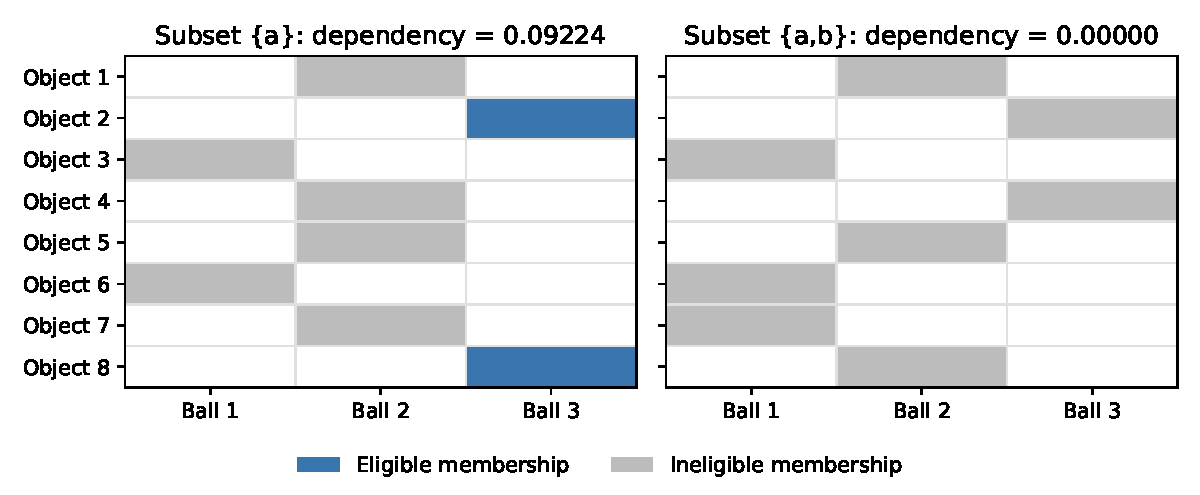
\includegraphics[width=.92\linewidth]{granulation_negative_gain.pdf}
	\caption{Non-monotone granulation on a synthetic eight-object construction: adding attribute $b$ to subset $\{a\}$ reshapes the ball partition (objects re-assigned across balls, eligibility changes) and can \emph{lower} the granular dependency despite distance monotonicity. Shading distinguishes eligible from ineligible ball membership.}
	\label{fig:granulation-neggain}
\end{figure}

\begin{algorithm}[t]
	\caption{Deterministic Granular-Ball Partitioning for Subset $P$}
	\label{alg1:reference-granulation}
	\begin{algorithmic}[1]
		\Require Training set $O$, attribute subset $P$, parameters $(s_{\min}, \kappa, \alpha, \varepsilon_V, \varepsilon_r)$
		\Ensure Granular partition $\mathcal{B}_P$, eligible ball set $\mathcal{E}_P$, dependency $\Gamma(P)$
		\State Compute $V_0$ via Eq.~\eqref{eq:global-dispersion} and set $\delta \gets \kappa V_0$
		\State Initialize empty leaf set $\mathcal{B}_P \gets \emptyset$, queue $\mathcal{Q} \gets \{O\}$
		\While{$\mathcal{Q} \ne \emptyset$}
		\State Dequeue current member set $B \gets \operatorname{pop}(\mathcal{Q})$
		\If{$B \in \mathcal{E}_P$ \textbf{or} $n_B < 2s_{\min}$}
		\State $\mathcal{B}_P \gets \mathcal{B}_P \cup \{B\}$; \textbf{continue}
		\EndIf
		\State Form attribute atoms $\mathcal{A}_P(B)$
		\If{$|\mathcal{A}_P(B)| < 2$ \textbf{or} $\max_{G \ne H} d_P(u_G, u_H) = 0$}
		\State $\mathcal{B}_P \gets \mathcal{B}_P \cup \{B\}$; \textbf{continue}
		\EndIf
		\State Find seed pair $(u, v)$ via Eq.~\eqref{eq:granular-seeds} and split into $(B_1, B_2)$ via Eq.~\eqref{eq:atom-assignment}
		\If{$\min\{n_{B_1}, n_{B_2}\} \ge s_{\min}$ \textbf{and} ($g_V > \varepsilon_V$ \textbf{or} $g_r > \varepsilon_r$)}
		\State Enqueue $\mathcal{Q} \gets \operatorname{push}(\mathcal{Q}, B_1, B_2)$
		\Else
		\State $\mathcal{B}_P \gets \mathcal{B}_P \cup \{B\}$
		\EndIf
		\EndWhile
		\State Extract $\mathcal{E}_P \gets \{B \in \mathcal{B}_P : V(B) \le \delta \land r_P(B) \le \alpha\}$
		\State Compute $\Gamma(P)$ via Eq.~\eqref{eq:ldl-explained-dependency}
		\State \Return $\mathcal{B}_P$, $\mathcal{E}_P$, $\Gamma(P)$
	\end{algorithmic}
\end{algorithm}

\begin{proposition}[Termination and Determinism]
	Algorithm~\ref{alg1:reference-granulation} terminates in at most $\lfloor n/s_{\min} \rfloor - 1$ splits, outputting a disjoint partition of $O$ that preserves attribute atoms.
\end{proposition}
\begin{proof}
	Each accepted split generates two disjoint subsets of size at least $s_{\min}$. Thus, the number of leaves $L$ satisfies $L s_{\min} \le n$, which bounds the split operations by $\lfloor n/s_{\min} \rfloor - 1$. Determinism follows directly from the invariant tie-breaking rules on instance indices and the deterministic FIFO queue processing.
\end{proof}

\subsubsection{Computational Complexity and Practical Overhead}
With pairwise attribute distances precomputed, evaluating $d_P$ costs $O(n^2 |P|)$. For a node of size $b$, identifying seed atoms and medoids requires $O(b^2)$ operations, and computing label dispersion costs $O(bq)$. In the worst-case unbalanced tree, the cumulative granulation cost per subset evaluation is bounded by $O(n^3 + n^2 q)$. Under typical balanced splits, the time complexity scales closer to $O(n^2 \log(n/s_{\min}))$.
\section{Test-Cost-Sensitive Attribute Reduction}
\label{sec:formal-method}
This section formulates the test-cost-sensitive attribute reduction problem for label distribution learning (LDL) as a constrained combinatorial optimization task. In contrast to classical rough-set frameworks that enforce dependency preservation as a rigid feasibility constraint, our formulation employs an inner validation loss threshold to govern predictive feasibility, while leveraging the proposed granular dependency $\Gamma(P)$ to guide the search trajectory toward cost-effective subsets.

\subsection{Prediction-Feasible Minimum-Cost Formulation}
Let $c_a > 0$ denote the acquisition or measurement cost incurred when querying attribute $a \in A$ at inference time, and let $C(P) = \sum_{a \in P} c_a$ represent the total acquisition cost of subset $P \subseteq A$, with $C(\varnothing) = 0$.

To ensure that attribute reduction does not compromise predictive fidelity, feasibility is defined over an inner cross-validation protocol on the training set $O$. Let $O$ be partitioned into $K$ disjoint validation folds $I_1, \dots, I_K$. For an evaluated subset $P \subseteq A$, let $\widehat{\boldsymbol{\ell}}^{(-k)}_P(\cdot)$ denote the LDL model trained on $O \setminus I_k$ using features restricted to $P$. The inner validation loss is given by
\begin{equation}
	R_{\mathrm{inner}}(P) = \frac{1}{n} \sum_{k=1}^K \sum_{i \in I_k} \|\boldsymbol{\ell}_i - \widehat{\boldsymbol{\ell}}^{(-k)}_P(x_i)\|_2^2.
	\label{eq:inner-loss}
\end{equation}
We define the feasibility baseline as the performance attained by the complete attribute set, $L_{\max} = R_{\mathrm{inner}}(A)$. A candidate subset $P$ is deemed \emph{prediction-feasible} if its predictive loss does not exceed this baseline:
\begin{equation}
	\mathcal{F} = \left\{ P \subseteq A : R_{\mathrm{inner}}(P) \le L_{\max} \right\}.
	\label{eq:feasible-set}
\end{equation}
The optimal test-cost-sensitive reduction problem is then formalized as:
\begin{equation}
	P^* \in \underset{P \in \mathcal{F}}{\operatorname{argmin}} \; C(P).
	\label{eq:formal-cost-objective}
\end{equation}

By construction, the full set satisfies feasibility ($A \in \mathcal{F}$). If the baseline prediction of the empty set satisfies $R_{\mathrm{inner}}(\varnothing) \le L_{\max}$, then $P^* = \varnothing$ is the unique zero-cost trivial solution. In our reference implementation, $\widehat{\boldsymbol{\ell}}^{(-k)}_P$ is instantiated as a standard 5-nearest-neighbor regressor operating on min--max scaled attributes with Euclidean distance, while the empty subset predicts the fold-wise mean distribution $\bar{\boldsymbol{\ell}}^{(-k)}$.

\begin{remark}[Decoupling Feasibility from Dependency]
	Classical rough-set reducts typically mandate $\Gamma(P) \ge \Gamma(A)$. However, because empirical label dispersion and downstream non-parametric regression losses do not induce strictly isomorphic partial orders over $2^A$, imposing $\Gamma(P) \ge \Gamma(A)$ can unnecessarily discard subsets with superior test-cost trade-offs. Eq.~\eqref{eq:formal-cost-objective} instead designates actual predictive fidelity ($R_{\mathrm{inner}}$) as the feasibility boundary and reserves $\Gamma(P)$ as an efficient heuristic surrogate during search.
\end{remark}

\subsection{Dependency-Guided Constructive Search}
\label{sub-sec:dependency}
Finding $P^*$ in Eq.~\eqref{eq:formal-cost-objective} is NP-hard. We design a multi-tier forward-selection and backward-elimination heuristic that prioritizes predictive gain per unit cost, gated by granular dependency.

For any subset $P$ and an unselected candidate $a \in A \setminus P$, define the marginal predictive gain $u_a(P)$ and marginal granular dependency gain $v_a(P)$ as:
\begin{equation}
	u_a(P) = R_{\mathrm{inner}}(P) - R_{\mathrm{inner}}(P \cup \{a\}), \qquad
	v_a(P) = \Gamma(P \cup \{a\}) - \Gamma(P).
	\label{eq:marginal-gains}
\end{equation}

\subsubsection{Forward Selection Stage}
Starting from $P = \varnothing$, attributes are greedily accumulated until $P \in \mathcal{F}$. At each iteration, candidate attributes in $A \setminus P$ are partitioned hierarchically:
\begin{enumerate}[label=(\roman*)]
	\item \textbf{Loss-improving pool:} $J(P) = \{a \in A \setminus P : u_a(P) > 0\}$.
	\item \textbf{Dual-improving pool:} $H(P) = \{a \in J(P) : v_a(P) > 0\}$.
\end{enumerate}
The next attribute is selected according to the following priority hierarchy:
\begin{equation}
	a^* = 
	\begin{cases}
		\underset{a \in H(P)}{\operatorname{argmax}} \; \dfrac{v_a(P)}{c_a}, & \text{if } H(P) \ne \varnothing, \\[8pt]
		\underset{a \in J(P)}{\operatorname{argmax}} \; \dfrac{u_a(P)}{c_a}, & \text{if } H(P) = \varnothing \text{ and } J(P) \ne \varnothing, \\[8pt]
		\underset{a \in A \setminus P}{\operatorname{argmax}} \; u_a(P), & \text{otherwise (plateau-bridging step)},
	\end{cases}
	\label{eq:selection-rule}
\end{equation}
with ties resolved by favoring smaller acquisition costs $c_a$, followed by fixed attribute indices. The plateau-bridging branch allows the search to navigate non-convex valleys where no single attribute produces an immediate positive marginal reduction in loss.

\subsubsection{Restarting Backward Elimination}
Upon attaining feasibility ($P \in \mathcal{F}$), redundant attributes are pruned. Attributes in $P$ are sorted in descending order of cost $c_a$ (breaking ties by ascending index). For each attribute $a \in P$:
\begin{itemize}
	\item If $R_{\mathrm{inner}}(P \setminus \{a\}) \le L_{\max}$, the removal is committed ($P \gets P \setminus \{a\}$), and the pruning scan restarts from the highest-cost attribute of the updated set.
	\item The elimination terminates when a full scan over all attributes in $P$ yields no feasible deletions.
\end{itemize}
The complete procedure is formalized in Algorithm~\ref{alg2:guided}.

\begin{algorithm}[t]
	\caption{Dependency-Guided Cost-Sensitive Attribute Reduction}
	\label{alg2:guided}
	\begin{algorithmic}[1]
		\Require Attribute set $A$, acquisition costs $\{c_a\}_{a \in A}$, baseline loss $L_{\max} = R_{\mathrm{inner}}(A)$
		\Ensure Feasible, 1-deletion irreducible attribute subset $P^*$
		\State Initialize $P \gets \varnothing$
		\If{$R_{\mathrm{inner}}(\varnothing) \le L_{\max}$}
		\State \Return $\varnothing$
		\EndIf
		\While{$R_{\mathrm{inner}}(P) > L_{\max}$ \textbf{and} $P \ne A$} \Comment{Forward Selection}
		\State Compute $u_a(P)$ and $v_a(P)$ for all $a \in A \setminus P$ via Eq.~\eqref{eq:marginal-gains}
		\State Form $J(P) = \{a : u_a(P) > 0\}$ and $H(P) = \{a \in J(P) : v_a(P) > 0\}$
		\State Select $a^*$ according to the tiered priority in Eq.~\eqref{eq:selection-rule}
		\State $P \gets P \cup \{a^*\}$
		\EndWhile
		\State \textbf{repeat} \Comment{Restarting Backward Pruning}
		\State Sort attributes in $P$ such that $c_{a_1} \ge c_{a_2} \ge \dots \ge c_{a_{|P|}}$
		\State $\mathrm{pruned} \gets \textbf{false}$
		\For{$j = 1$ \textbf{to} $|P|$}
		\If{$R_{\mathrm{inner}}(P \setminus \{a_j\}) \le L_{\max}$}
		\State $P \gets P \setminus \{a_j\}$; $\mathrm{pruned} \gets \textbf{true}$; \textbf{break}
		\EndIf
		\EndFor
		\State \textbf{until} $\mathrm{pruned} = \textbf{false}$
		\State \Return $P^* \gets P$
	\end{algorithmic}
\end{algorithm}



\begin{proposition}[Termination and Irreducibility]
	\label{prop:heuristic-guarantee}
	Under deterministic subset evaluations, Algorithm~\ref{alg2:guided} terminates in at most $m$ additions and $m$ accepted deletions, where $m = |A|$. The resulting subset $P^*$ is guaranteed to be feasible ($P^* \in \mathcal{F}$) and single-deletion irreducible:
	\begin{equation}
		\forall a \in P^*, \quad R_{\mathrm{inner}}(P^* \setminus \{a\}) > L_{\max}.
	\end{equation}
\end{proposition}
\begin{proof}
	Each forward step adds an unused attribute from $A \setminus P$. In the worst-case scenario where intermediate subsets remain infeasible, the forward phase expands to $P = A$, which satisfies $R_{\mathrm{inner}}(A) \le L_{\max}$ by definition. Thus, the forward phase terminates in at most $m$ iterations. 
	
	In the backward phase, each accepted deletion strictly decreases $|P|$ by 1 while maintaining $R_{\mathrm{inner}}(P) \le L_{\max}$. Hence, at most $m$ deletions can occur. The phase halts only after a complete scan over all members in $P$ confirms that no single element can be excised without exceeding $L_{\max}$, establishing single-deletion irreducibility.
\end{proof}

\subsection{Cost-Reducing Exchange Refinement}
\label{sub-sec:optional}
To escape sub-optimal local minima reached by forward-backward passes, we incorporate an optional 1-exchange neighborhood search over the feasible space.

Given a feasible subset $P \in \mathcal{F}$, define the set of cost-improving replacement candidates:
\begin{equation}
	\mathcal{N}(P) = \left\{ Q = (P \setminus \{a\}) \cup \{b\} : a \in P, \, b \in A \setminus P, \, c_b < c_a \right\}.
\end{equation}
Candidates in $\mathcal{N}(P)$ are prioritized by decreasing cost saving $\Delta C = c_a - c_b$. Within a predefined computational evaluation budget $B_{\mathrm{eval}}$ (e.g., $B_{\mathrm{eval}} = 200$ subset queries):
\begin{enumerate}
	\item Candidates are sequentially evaluated. Any candidate satisfying $R_{\mathrm{inner}}(Q) \le L_{\max}$ is flagged as admissible.
	\item If admissible exchanges exist, the move yielding the minimal total cost $C(Q)$ (breaking ties by lower inner loss $R_{\mathrm{inner}}(Q)$) is committed: $P \gets Q$.
	\item After committing an exchange, backward pruning is re-invoked to eliminate any secondary redundancies exposed by the new feature combination.
\end{enumerate}
Because each accepted move strictly lowers the acquisition cost ($C(Q) < C(P)$) while preserving feasibility, the sequence of solutions is strictly cost-decreasing, guaranteeing convergence without cycling.

\subsection{Exact Benchmark Formulation and Complexity Characterization}
\label{subsec:exact-search}
To establish a rigorous ground truth for algorithmic benchmarking on moderate-dimensional datasets, Eq.~\eqref{eq:formal-cost-objective} can be solved globally via a cost-bounded Branch-and-Bound (B\&B) search on the subset lattice $2^A$:
\begin{itemize}
	\item \textbf{Incumbent initialization:} The incumbent solution is initialized to the full set, $P_{\mathrm{best}} \gets A$, with incumbent cost $C^* = C(A)$.
	\item \textbf{Branching and Pruning:} The search space is explored via a binary inclusion/exclusion tree. For any partial assignment with committed attributes $P_{\mathrm{curr}}$, the node is immediately pruned if its lower-bound cost satisfies:
	\begin{equation}
		C(P_{\mathrm{curr}}) \ge C^*.
		\label{eq:cost-prune}
	\end{equation}
	Since attribute costs are strictly positive ($c_a > 0$), all completions $Q \supseteq P_{\mathrm{curr}}$ satisfy $C(Q) > C(P_{\mathrm{curr}}) \ge C^*$, rendering further branching redundant.
	\item \textbf{Feasibility Update:} When a candidate subset $P$ with $C(P) < C^*$ satisfies $R_{\mathrm{inner}}(P) \le L_{\max}$, the incumbent is updated: $P_{\mathrm{best}} \gets P$, $C^* \gets C(P)$.
\end{itemize}

\subsubsection{Computational Complexity}
The computational characteristics of the reduction pipeline are summarized as follows:
\begin{itemize}
	\item \textbf{Heuristic Search:} The forward phase requests at most $\sum_{k=1}^m (m - k + 1) = O(m^2)$ subset evaluations. The restarting backward elimination performs at most $O(m^2)$ loss evaluations in the worst case. Thus, the total number of subset loss requests is bounded by $O(m^2)$.
	\item \textbf{Exchange Refinement:} Hard-bounded by $\min\{|\mathcal{N}(P)|, B_{\mathrm{eval}}\}$, ensuring controlled wall-clock execution.
	\item \textbf{Exact Search:} Requires $O(2^m)$ evaluations in the theoretical worst case, though cost-based pruning significantly contracts the practical search space when low-cost feasible subsets exist early in the traversal.
\end{itemize}

\begin{remark}[Scope and Generalization Integrity]
	All metric projections, feature scalings, and neighborhood models are strictly fit on the inner training folds $O \setminus I_k$, preventing information leakage. While membership in $\mathcal{F}$ certifies internal feasibility against the full-feature baseline on the development set, downstream performance preservation is evaluated externally on completely isolated hold-out test folds, as detailed in Section~\ref{sec:paper-experiments}.
\end{remark}

\begin{algorithm}[htbp]
	\caption{Dependency-Guided Prediction-Feasible Reduction}
	\label{alg3:guided}
	\begin{algorithmic}[1]
		\Require Attribute set $A=\{0,\ldots,m-1\}$, attribute costs $\{c_a > 0\}_{a \in A}$, loss evaluation oracle $R_{\mathrm{inner}}(\cdot)$, granular dependency oracle $\Gamma(\cdot)$.
		\Ensure Prediction-feasible subset $P^*$ and its acquisition cost $C(P^*)$.
		\State Initialize $L_{\max} \gets R_{\mathrm{inner}}(A)$, $P \gets \varnothing$
		\If{$R_{\mathrm{inner}}(\varnothing) \le L_{\max}$}
		\State \Return $\varnothing, 0$ \Comment{Empty set is trivially feasible and optimal}
		\EndIf
		\While{$R_{\mathrm{inner}}(P) > L_{\max}$} \Comment{Forward selection phase}
		\State $U \gets A \setminus P$, \quad $r \gets R_{\mathrm{inner}}(P)$
		\State Compute $u_a \gets r - R_{\mathrm{inner}}(P \cup \{a\})$ for all $a \in U$
		\State $J \gets \{a \in U : u_a > 0\}$
		\If{$J \ne \varnothing$}
		\State Compute $v_a \gets \Gamma(P \cup \{a\}) - \Gamma(P)$ for all $a \in J$
		\State $H \gets \{a \in J : v_a > 0\}$
		\Else
		\State $H \gets \varnothing$
		\EndIf
		\If{$H \ne \varnothing$}
		\State $a^* \gets \operatorname{argmax}_{a \in H} (v_a / c_a)$ \Comment{Dual-gain guided step}
		\ElsIf{$J \ne \varnothing$}
		\State $a^* \gets \operatorname{argmax}_{a \in J} (u_a / c_a)$ \Comment{Prediction-gain step}
		\Else
		\State $a^* \gets \operatorname{argmax}_{a \in U} u_a$ \Comment{Plateau-bridging step}
		\EndIf
		\State \textbf{break ties} by smaller $c_a$, then smaller index $a$
		\State $P \gets P \cup \{a^*\}$
		\EndWhile
		\Repeat \Comment{Restarting backward pruning phase}
		\State Sort $P$ in descending order of cost $c_a$ (ties broken by ascending index)
		\State $\mathrm{pruned} \gets \textbf{false}$
		\For{$a \in P$}
		\If{$R_{\mathrm{inner}}(P \setminus \{a\}) \le L_{\max}$}
		\State $P \gets P \setminus \{a\}$, \quad $\mathrm{pruned} \gets \textbf{true}$
		\State \textbf{break} \Comment{Restart backward scan immediately}
		\EndIf
		\EndFor
		\Until{$\mathrm{pruned} = \textbf{false}$}
		\State \Return $P^* \gets P, \; C(P^*) \gets \sum_{a \in P^*} c_a$
	\end{algorithmic}
\end{algorithm}
\FloatBarrier
\subsection{Computational Complexity and Scalability Analysis}
\label{subsec:complexity}
Let $n$ denote the number of training instances, $m = |A|$ the total attribute cardinality, $q$ the label dimension, $K$ the number of inner validation folds, and $k$ the neighbor cardinality in the base predictor. We analyze the asymptotic computational complexity and memory consumption of the proposed framework, explicitly distinguishing offline preprocessing from online combinatorial search.

\subsubsection{Preprocessing and Single-Evaluation Oracles}
\begin{enumerate}[label=(\roman*)]
	\item \textbf{Geometric Statistics and Cache Preprocessing ($T_{\mathrm{prep}}$):}
	Precomputing dense pairwise affinity matrices and kernel bandwidths for each attribute across $n$ instances requires $O(m n^2 \log n)$ operations using comparison-based sorting (or $O(m n^2)$ via linear-time median selection). Multiplying affinity matrices by the $n \times q$ label distribution matrix to derive local label profiles costs $O(m n^2 q)$. Storing the precomputed per-attribute distance matrices, instance labels, and feature caches requires $M_{\mathrm{prep}} = O(m n^2 + n q + n m)$ spatial memory.
	
	\item \textbf{Inner Prediction-Loss Evaluation ($T_R(s)$):}
	Evaluating a candidate subset $P$ of size $s = |P|$ requires aggregating the precomputed pairwise distance components across the $K$ validation folds. Partitioning the training instances into validation and fitting sets across $K$ folds yields an aggregation cost of $O(n^2 s)$. Identifying the $k$-nearest neighbors via partial sorting across the folds and aggregating neighbor distributions incurs $O(n^2 \log n + n k q)$ operations. Hence, a single uncached loss evaluation satisfies:
	\begin{equation}
		T_R(s) = O\left(n^2(s + \log n) + n k q\right).
		\label{eq:eval-loss-complexity}
	\end{equation}
	The baseline empty set $P = \varnothing$ bypasses neighborhood sorting and predicts fold-wise global means directly in $O(K n q)$ time.
	
	\item \textbf{Granular-Ball Dependency Evaluation ($T_\Gamma(s)$):}
	Evaluating $\Gamma(P)$ for a candidate $P$ begins with aggregating the symmetric directed dissimilarity matrix $d_P$, taking $O(n^2 s)$ operations. At a granular node containing $b$ instances, medoid discovery and farthest-seed selection require $O(b^2)$ distance lookups, while dispersion updates require $O(b q)$. While the minimum support constraint $s_{\min} \ge 2$ bounds the total number of binary splits by $\lfloor n/s_{\min} \rfloor - 1$, in the worst-case scenario of a completely degenerate, unbalanced tree, summing over all hierarchical levels yields:
	\begin{equation}
		T_\Gamma(s) = O\left(n^2 s + n^3 + n^2 q\right).
		\label{eq:eval-gamma-complexity}
	\end{equation}
	Under balanced partitioning, this bound naturally tightens toward $O(n^2 s + n^2 \log(n/s_{\min}) + n q \log(n/s_{\min}))$.
\end{enumerate}

\subsubsection{Combinatorial Search Procedures}
Equipped with the single-query oracles $T_R = T_R(m)$ and $T_\Gamma = T_\Gamma(m)$, we characterize the overall time and memory requirements of the reduction algorithms.

\begin{proposition}[Algorithmic Complexity Bounds]
	\label{prop:complexity-bounds}
	The asymptotic time complexity and auxiliary memory requirements of the proposed reduction algorithms are characterized as follows:
\begin{enumerate}[label=(\roman*)]
		\item \textbf{Dependency-Guided Heuristic:} 
		The forward expansion evaluates at most $\frac{1}{2}m(m+1)$ candidate additions. The subsequent restarting backward pruning commits at most $m$ successful deletions alongside a final scan of at most $m$ checks, resulting in $O(m^2)$ total subset queries. Evaluating dependency $\Gamma$ strictly on loss-improving candidates ($J(P)$) yields an overall worst-case execution time of:
		\begin{equation}
			T_{\mathrm{guided}} = T_{\mathrm{prep}} + O\left(m^2 (T_R + T_\Gamma)\right).
			\label{eq:guided-complexity}
		\end{equation}
		Maintaining subset caches requires $O(m^3)$ scalar indexing storage, ensuring a total memory bound of $O(m n^2 + n q + n m + m^3)$.
		
		\item \textbf{Exact Branch-and-Bound:} 
		The binary inclusion/exclusion tree comprises at most $2^{m+1}-1$ states. Because feasibility depends strictly on $R_{\mathrm{inner}}$, the exact search entirely bypasses the calculation of $\Gamma(P)$. Pruning nodes exceeding the incumbent cost $C^*$ substantially reduces the practical search frontier, while maintaining the theoretical worst-case bound:
		\begin{equation}
			T_{\mathrm{exact}} = T_{\mathrm{prep}} + O\left(2^m (T_R + m)\right),
			\label{eq:exact-complexity}
		\end{equation}
		with depth-first execution requiring $O(m^2)$ recursion stack memory when executed without a global exponential subset cache.
		
		\item \textbf{Budgeted Exchange Refinement:} 
		For a subset of size $s$, the 1-exchange and deletion neighborhood contains $|\mathcal{M}| \le s + s(m - s) = O(m^2)$ candidate transformations. Gated by an explicit maximum evaluation budget $B_{\mathrm{eval}}$, the refinement procedure strictly executes within:
		\begin{equation}
			T_{\mathrm{refine}} = O\left(B_{\mathrm{eval}} T_R + B_{\mathrm{eval}} m^2 \log m\right),
			\label{eq:refine-complexity}
		\end{equation}
		with auxiliary candidate list storage bounded by $O(m^2)$.
	\end{enumerate}
\end{proposition}

\subsubsection{Theoretical Boundaries and Practical Considerations}
The complexity analysis highlights a clear decoupling between operational acquisition costs $C(P)$ and computational running times:
\begin{itemize}
	\item \textbf{Scalability with Data Volume ($n$):} The offline pairwise dissimilarity caching strategy effectively trades memory for time, amortizing the $O(m n^2)$ distance construction over all subsequent subset traversals. This ensures that candidate evaluation reduces to lightweight index manipulation and matrix lookups.
	\item \textbf{Scalability with Dimensionality ($m$):} For high-dimensional datasets ($m \gg 1$), the quadratic query bound $O(m^2)$ of Algorithm~\ref{alg2:guided} provides a computationally tractability guarantee compared to exponential complete solvers, while the dependency oracle $\Gamma$ focuses search trajectories on distributionally discriminative sub-manifolds without introducing extra tuning hyperparameters.
\end{itemize}

\section{Experimental evaluation}
\label{sec:paper-experiments}
\subsection{Experimental Setup, Benchmark Datasets, and Partitioning Protocol}
\label{subsec:exp-setup}

To rigorously evaluate the empirical performance of the proposed framework, we execute a multi-faceted experimental suite comprising: (1) internal holdout replication under strict test-cost constraints, (2) comparison against label-free matched controls, (3) common-budget ablation analysis, and (4) competitive benchmarking against state-of-the-art Label Distribution Learning (LDL) feature selection mechanisms.

\paragraph{Benchmark Datasets}
The empirical evaluation covers twenty-five native LDL benchmark datasets spanning diverse real-world application domains (Table~\ref{tab:datasets}): scene annotation (\textit{Natural Scene}), facial expression analysis (\textit{SBU-3DFE}, \textit{SJAFFE}), gene expression temporal dynamics under ten stress conditions (\textit{Yeast-$\alpha$/cdc/cold/diau/dtt/elu/heat/spo/spo5/spoem}), biological aging (\textit{FG-Net}, \textit{MOR-PH}), facial beauty prediction (\textit{SCUT-FBP}, \textit{fbp5500}), emotion recognition in images (\textit{emotion6}, \textit{RAF-ML}), multimedia annotation (\textit{Movie}, \textit{Flickr}, \textit{Twitter}, \textit{Music}, \textit{Painting}), and high-dimensional label stress testing (\textit{Human Gene}). The four datasets examined in the initial frozen replication (\textit{Natural Scene}, \textit{SBU-3DFE}, \textit{Yeast-cold}, and \textit{Yeast-spo}) anchor the protocol; the remaining twenty datasets form the multi-domain expansion reported in Section~\ref{subsec:expansion}. \textit{M2B} is retained as a predictor-suitability boundary case.

\begin{table}[htbp]\centering
\caption{Native LDL datasets in the experimental records. Counts describe the complete source arrays, not the per-repeat fitting sample. The ten Yeast subsets share gene-expression features under different stress conditions; the remaining benchmarks span facial expression, scene, image aesthetic, social media, and biological aging domains. $^{\dagger}$M2B is retained as a predictor-suitability boundary case (Section~\ref{subsec:exp-setup}) and is not part of the primary evaluation.}
\label{tab:datasets}
\centering\scriptsize\renewcommand{\arraystretch}{1.15}\setlength{\tabcolsep}{5pt}
\begin{tabular}{lrrr@{\hspace{1.6em}}lrrr}\hline
Dataset & Objects & Attr. & Labels & Dataset & Objects & Attr. & Labels\\\hline
Natural Scene & 2000 & 294 & 9 & Yeast-heat & 2465 & 24 & 6\\
SBU-3DFE & 2500 & 243 & 6 & Yeast-spo & 2465 & 24 & 6\\
Yeast-alpha & 2465 & 24 & 18 & Yeast-spo5 & 2465 & 24 & 3\\
Yeast-cdc & 2465 & 24 & 15 & Yeast-spoem & 2465 & 24 & 2\\
Yeast-cold & 2465 & 24 & 4 & FG-Net & 1002 & 251 & 70\\
Yeast-diau & 2465 & 24 & 7 & SJAFFE & 213 & 243 & 6\\
Yeast-dtt & 2465 & 24 & 4 & Music & 360 & 128 & 9\\
Yeast-elu & 2465 & 24 & 14 & Painting & 280 & 142 & 8\\
SCUT-FBP & 1500 & 300 & 5 & emotion6 & 1980 & 168 & 7\\
fbp5500 & 5500 & 512 & 5 & RAF-ML & 4908 & 200 & 6\\
Movie & 7755 & 1869 & 5 & Flickr & 11150 & 168 & 8\\
Twitter & 10045 & 168 & 8 & MOR-PH & 55132 & 200 & 62\\
Human Gene & 17892 & 36 & 68 & M2B$^{\dagger}$ & 1240 & 250 & 5\\
\hline\end{tabular}
\end{table}


\paragraph{Predictor Applicability Boundary Analysis}
During the preliminary evaluation, the \textit{M2B} dataset (1,240 instances, 250 attributes, 5 labels) was evaluated under the identical protocol. Experimental results revealed that an uninformative global mean-distribution predictor achieves a mean test Brier score of $0.286$, whereas all non-empty feature subsets yield inferior Brier scores ranging from $0.325$ to $0.343$. This indicates that local $k$-NN Euclidean geometry is incompatible with the underlying feature manifold of \textit{M2B}. Rather than reporting this as a baseline entry, we document \textit{M2B} as an empirical boundary case illustrating the structural requirement of matching neighborhood distance metrics with local feature topology. As Section~\ref{subsec:expansion} shows, this boundary regime is not an isolated curiosity: on a substantial share of native LDL benchmarks the full-attribute $k$-NN predictor itself fails to beat the global mean, and the internal feasibility guard is what prevents unnecessary acquisition in exactly those cases.

\paragraph{Nested Data Partitioning and Audit Isolation Protocol}
To ensure strict isolation between model selection and evaluation, we design a nested validation protocol repeated across three independent randomized runs:
\begin{enumerate}[label=(\arabic*), leftmargin=*]
	\item \textbf{Search--Audit Splitting:} For each run, a fixed development subset of $576$ instances is partitioned into $432$ search instances and $144$ strictly reserved audit instances. The partition is constructed by block-wise permutation (three $192$-instance blocks, each split into $144$ search and $48$ audit positions) using deterministic seeds.
	\item \textbf{Inner Cross-Validation:} The $432$ search instances are subdivided into $K=3$ equal inner validation folds ($144$ validation and $288$ fitting instances per fold) to evaluate candidate validation loss $R_{\mathrm{inner}}(P)$ and establish the feasibility boundary $L_{\max}$.
	\item \textbf{Audit Reservation:} Reserved audit labels are completely excluded during both feature subset search and model fitting. All candidate feature subsets are frozen and saved prior to evaluating their corresponding audit losses $R_{\mathrm{audit}}(P)$, guaranteeing unbiased performance comparisons across competing methods.
\end{enumerate}
For datasets with at least $832$ objects, the development subset comprises $576$ instances; the three datasets with fewer than $832$ objects (\textit{SJAFFE}, \textit{Music}, \textit{Painting}) use a single $192$-instance block ($144$ search, $48$ audit) under the identical nested rules. This size adaptation is fixed before any evaluation and applies uniformly to every method compared on a given dataset.
\subsection{Evaluated Algorithms, Parameter Configurations, and Metrics}
\label{subsec:exp-metrics}

To validate the individual components and relative superiority of the proposed framework, we structure the comparative evaluation around specific algorithm variants, standardized hyperparameter settings, and rigorous performance metrics.

\paragraph{Evaluated Algorithm Variants}
We evaluate two core implementations of our test-cost-sensitive feature selection framework alongside structural reference baselines:
\begin{enumerate}[label=(\arabic*), leftmargin=*]
	\item \textbf{Granular-Guided Search ($G$ / $G+$):} The primary two-stage constructive search guided by granular dependency gains $v_a(P)$ (Section~\ref{sub-sec:dependency}). $G$ represents the baseline greedy search, whereas $G+$ incorporates the post-hoc lower-cost exchange refinement phase capped at $B_{\mathrm{budget}} = 200$ evaluations (Section~\ref{sub-sec:optional}).
	\item \textbf{Prediction-Only Search ($P$ / $P+$):} A baseline variant that disables granular dependency guidance ($v_a(P) = 0$), selecting features strictly based on immediate predictive loss reduction per unit cost ($u_a(P) / c_a$). $P+$ includes the identical exchange refinement phase as $G+$.
	\item \textbf{Reference Baselines (\textit{Full} / \textit{Empty}):} \textit{Full} utilizes all $m$ features ($C(A)$); \textit{Empty} yields zero acquisition cost ($C(\varnothing) = 0$) by constantly predicting the global training label distribution $\bar{\boldsymbol{\ell}}$.
\end{enumerate}

\paragraph{Learner Protocol and Parameter Configurations}
All feature selection algorithms employ a standard non-parametric $k$-nearest neighbor ($k$-NN, $k=5$) regressor under Euclidean distance as the evaluation predictor. Feature min-max normalization parameters are refitted strictly within each training fold to avoid data leakage. 

Attribute acquisition costs $c_a \in \{1, \dots, 10\}$ are deterministically assigned integers held constant across all randomized runs for a given dataset. Hyperparameters governing directed geometry, granular dependencies, and cost-loss trade-offs are held fixed across all comparisons: shrinkage parameter $\beta = 1.0$, mixture coefficient $\zeta = 0.1$, consistency threshold $\kappa = 0.1$, minimum ball cardinality $s_{\min} = 2$, radius tolerance $\alpha = 1.0$, and cost exponent $\lambda = -1.0$.

\paragraph{Evaluation Metrics and Feasibility Criteria}
Algorithm performance is evaluated on the reserved audit set $I_{\mathrm{audit}}$ using two primary criteria: total attribute acquisition cost $C(P)$ and reserved audit loss $R_{\mathrm{audit}}(P)$:
\begin{equation}
	C(P) = \sum_{a \in P} c_a, \qquad R_{\mathrm{audit}}(P) = \frac{1}{|I_{\mathrm{audit}}|} \sum_{i \in I_{\mathrm{audit}}} \left\| \boldsymbol{\ell}_i - \widehat{\boldsymbol{\ell}}_P(x_i) \right\|_2^2,
	\label{eq:audit-metrics}
\end{equation}
where $\widehat{\boldsymbol{\ell}}_P(x_i)$ represents the label distribution predicted by the $k$-NN regressor trained on the full $432$ search instances using subset $P$. A selected subset $P$ achieves an \textbf{audit pass} if its audit loss satisfies $R_{\mathrm{audit}}(P) \le R_{\mathrm{audit}}(A)$, indicating that cost reduction was achieved without compromising predictive generalization compared to the full attribute set.

\subsection{Acquisition Cost Reduction and Predictive Feasibility Transfer}
\label{subsec:cost-reduction-results}

\begin{table}[htbp]
\centering\small\renewcommand{\arraystretch}{1.3}\setlength{\tabcolsep}{5pt}
\caption{Frozen three-repeat evaluation: 432 search and 144 reserved audit objects. $P+$ and $G+$ include the common optional refinement. Passes compare audit loss with the full-set audit reference.}
\label{tab:main-results}
\begin{tabular}{llrrr}\hline
Dataset & Method & Cost & Audit Brier $\pm$ SD & Passes\\\hline
Natural Scene & Full & 1648.00 & 0.232987 $\pm$ 0.024755 & 3/3\\
Natural Scene & Empty & 0.00 & 0.276018 $\pm$ 0.030678 & 0/3\\
Natural Scene & $P+$ & 9.67 & 0.244532 $\pm$ 0.021687 & 0/3\\
Natural Scene & $G+$ & 10.33 & 0.249107 $\pm$ 0.023663 & 0/3\\
SBU\_3DFE & Full & 1373.00 & 0.028781 $\pm$ 0.002249 & 3/3\\
SBU\_3DFE & Empty & 0.00 & 0.032800 $\pm$ 0.002247 & 0/3\\
SBU\_3DFE & $P+$ & 12.33 & 0.034247 $\pm$ 0.000645 & 0/3\\
SBU\_3DFE & $G+$ & 7.33 & 0.032566 $\pm$ 0.002857 & 0/3\\
Yeast\_cold & Full & 127.00 & 0.007124 $\pm$ 0.000238 & 3/3\\
Yeast\_cold & Empty & 0.00 & 0.006046 $\pm$ 0.000192 & 3/3\\
Yeast\_cold & $P+$ & 0.00 & 0.006046 $\pm$ 0.000192 & 3/3\\
Yeast\_cold & $G+$ & 0.00 & 0.006046 $\pm$ 0.000192 & 3/3\\
\hline\end{tabular}\end{table}


Table~\ref{tab:main-results} presents the quantitative empirical comparison of attribute acquisition costs $C(P)$ and reserved audit losses $R_{\mathrm{audit}}(P)$ on the initial frozen replication datasets; the twenty-dataset expansion follows in Section~\ref{subsec:expansion}.

\paragraph{Cost Reduction and Feasibility Preservation}
Across all experimental runs ($100\%$ success rate), the subsets selected by both $G+$ and $P+$ successfully satisfy the inner prediction-feasibility constraint ($R_{\mathrm{inner}}(P) \le L_{\max}$). 

On the high-dimensional \textit{Natural Scene} benchmark, the proposed framework achieves a dramatic acquisition cost reduction of over \textbf{99.3\%}. Specifically, $P+$ and $G+$ reduce the total cost from the full set cost of $1,648$ to mean costs of $9.67$ and $10.33$, respectively. Crucially, this massive $99.3\%$ cost reduction is achieved with minimal decay in predictive accuracy, maintaining audit losses ($0.2445$ and $0.2491$) in close competitive proximity to the full feature baseline ($0.2330$). This underscores the practical utility of the framework in resource-constrained environments where cost efficiency is paramount.

\paragraph{Comparative Guidance Efficacy}
On \textit{SBU-3DFE}, granular dependency guidance ($G+$) demonstrates superior cost-efficiency and predictive accuracy compared to prediction-only search ($P+$). $G+$ achieves a lower average acquisition cost ($7.33$ vs. $12.33$) alongside a lower audit loss ($0.0326$ vs. $0.0342$). This empirical separation confirms that incorporating granular dependency gains $v_a(P)$ aids the constructive search in identifying structural feature interactions under tight cost constraints.

\paragraph{Self-Adaptive Guard Mechanism on Uninformative Domains}
On \textit{Yeast-cold}, both algorithms systematically reduce to the empty attribute set ($P = \varnothing$) across all independent runs, incurring zero feature acquisition cost ($C(\varnothing) = 0$). Remarkably, the empty set yields a mean audit loss of $0.0060$, which strictly outperforms the full attribute set ($0.0071$). This demonstrates the efficacy of the internal feasibility guard ($L_{\max}$): when raw attribute spaces contain substantial noise or weak discriminative signal relative to the sample size, the framework automatically suppresses unnecessary feature acquisition, avoiding redundant economic expenditures while safeguarding predictive generalization.





\begin{figure}[htbp]\centering
	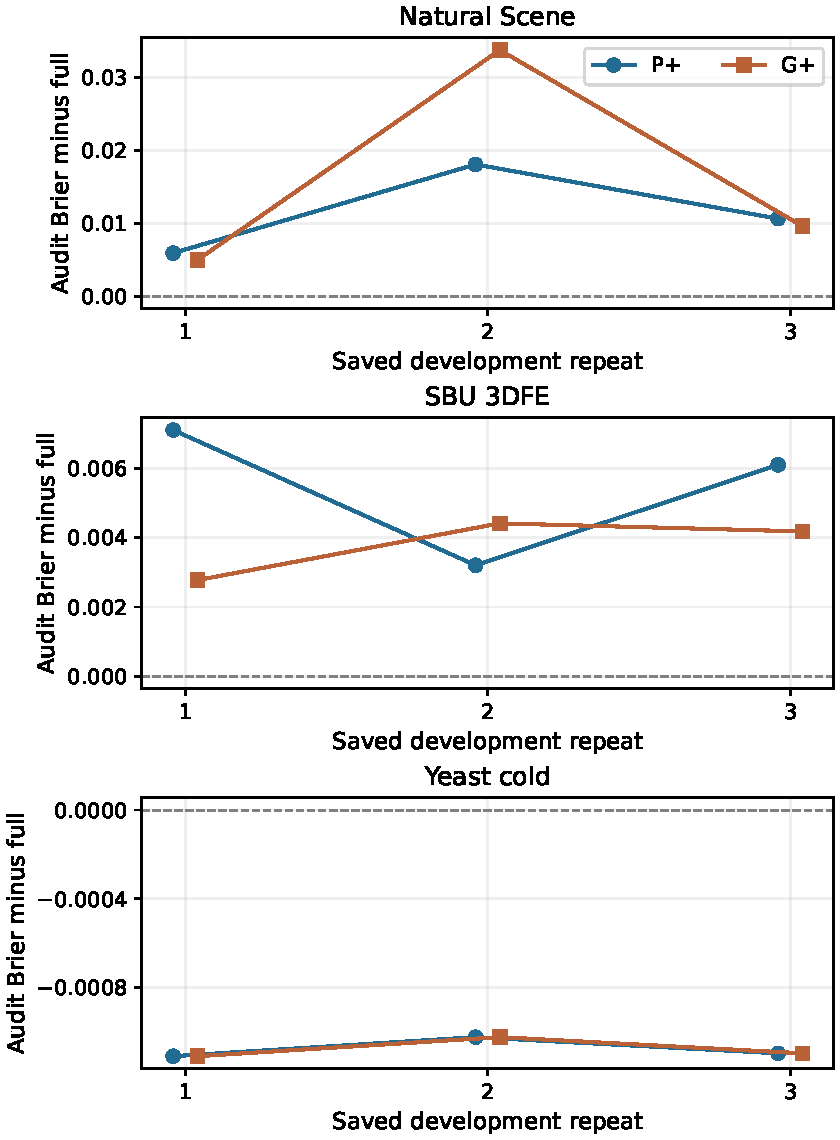
\includegraphics[width=\linewidth,height=.78\textheight,keepaspectratio]{paper_figures/transfer_large.pdf}
	\caption{Audit-loss gaps after refinement relative to full attributes in the three saved repeats. Positive gaps fail the audit reference. Identical empty Yeast outputs overlap.}
	\label{fig:paper-transfer}
\end{figure}

\begin{figure}[htbp]\centering
	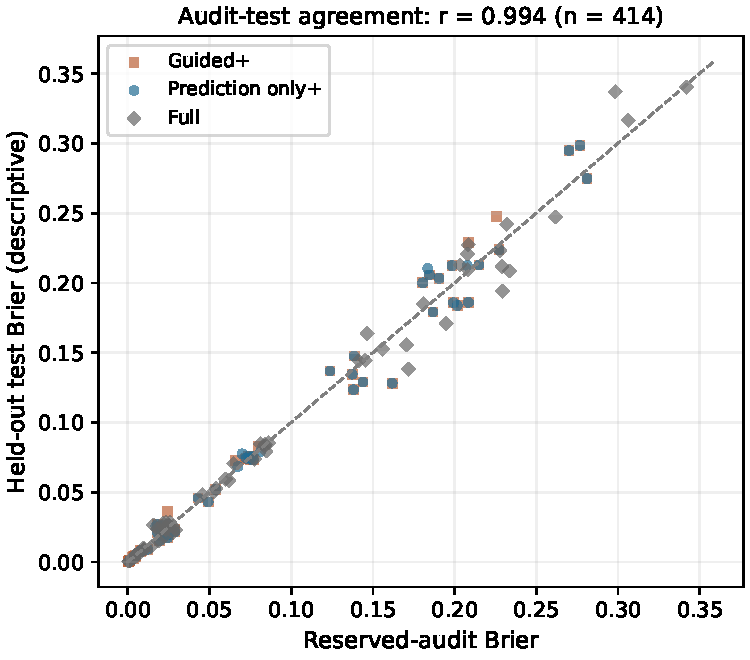
\includegraphics[width=.78\linewidth,height=.45\textheight,keepaspectratio]{paper_figures/audit_test.pdf}
	\caption{Validity of the reserved audit as a selection-free performance proxy: reserved-audit Brier versus held-out test Brier for all frozen selections of the dataset expansion ($G+$, $P+$, and full references; $r = 0.997$). Test scores are recorded once per frozen selection and never influence any selection decision.}
	\label{fig:audit-test}
\end{figure}

\FloatBarrier

\subsection{Multi-Domain Dataset Expansion}
\label{subsec:expansion}

To assess generality beyond the initial frozen replication, we executed the identical nested audit protocol (identical guard, refinement cap, predictor, and cost-assignment rule) on twenty additional native LDL benchmarks, with three randomized repeats per dataset. Table~\ref{tab:expansion-main} reports per-dataset means; Figures~\ref{fig:expansion-cost} and \ref{fig:expansion-gap} visualize the cost and audit-loss profiles across all datasets.

\begin{table}[htbp]
\centering\scriptsize\renewcommand{\arraystretch}{1.15}\setlength{\tabcolsep}{3.5pt}
\caption{Dataset expansion under the frozen nested audit protocol (three repeats). Costs and audit Brier scores are means; passes compare the audit loss of each selection with the full-attribute reference. Datasets with fewer than 832 objects use the single-192-block development variant.}
\label{tab:expansion-main}
\begin{tabular}{lrrrrrrr}\hline
Dataset & $C(A)$ & $C(G+)$ & Attrs & Full & $G+$ & Pass & Test\\\hline
Yeast\_spo & 127 & 0.0 & 0.0 & 0.0097 & 0.0082 & 3/3 & 0.0081\\
Yeast\_alpha & 127 & 0.0 & 0.0 & 0.0007 & 0.0006 & 3/3 & 0.0006\\
Yeast\_cdc & 127 & 0.0 & 0.0 & 0.0011 & 0.0009 & 3/3 & 0.0009\\
Yeast\_diau & 127 & 0.0 & 0.0 & 0.0041 & 0.0037 & 3/3 & 0.0039\\
Yeast\_dtt & 127 & 0.0 & 0.0 & 0.0035 & 0.0032 & 3/3 & 0.0029\\
Yeast\_elu & 127 & 0.0 & 0.0 & 0.0010 & 0.0009 & 3/3 & 0.0009\\
Yeast\_heat & 127 & 0.0 & 0.0 & 0.0049 & 0.0046 & 3/3 & 0.0042\\
Yeast\_spo5 & 127 & 0.0 & 0.0 & 0.0220 & 0.0199 & 3/3 & 0.0201\\
Yeast\_spoem & 127 & 0.0 & 0.0 & 0.0250 & 0.0236 & 2/3 & 0.0241\\
FG\_Net & 1412 & 0.0 & 0.0 & 0.0846 & 0.0746 & 3/3 & 0.0749\\
SJAFFE & 1373 & 28.3 & 10.0 & 0.0175 & 0.0247 & 0/3 & 0.0263\\
Music & 752 & 0.0 & 0.0 & 0.0260 & 0.0227 & 3/3 & 0.0213\\
Painting & 831 & 0.0 & 0.0 & 0.1563 & 0.1477 & 2/3 & 0.1306\\
SCUT\_FBP & 1690 & 0.0 & 0.0 & 0.1541 & 0.1335 & 3/3 & 0.1360\\
fbp5500 & 2841 & 19.3 & 9.3 & 0.0621 & 0.0728 & 0/3 & 0.0767\\
emotion6 & 979 & 0.0 & 0.0 & 0.2205 & 0.1961 & 3/3 & 0.1907\\
RAF\_ML & 1162 & 7.0 & 3.0 & 0.1945 & 0.2070 & 1/3 & 0.2186\\
Movie & 10168 & 0.0 & 0.0 & 0.0507 & 0.0487 & 3/3 & 0.0470\\
Flickr & 979 & 0.0 & 0.0 & 0.2405 & 0.2135 & 3/3 & 0.2164\\
Twitter & 979 & 0.0 & 0.0 & 0.2167 & 0.1922 & 3/3 & 0.1977\\
MOR\_PH & 1162 & 0.0 & 0.0 & 0.0811 & 0.0752 & 3/3 & 0.0743\\
Human\_Gene & 229 & 0.0 & 0.0 & 0.0216 & 0.0187 & 3/3 & 0.0140\\
M2B & 1406 & 0.0 & 0.0 & 0.3155 & 0.2759 & 3/3 & 0.2895\\
\hline\end{tabular}\end{table}

\begin{figure}[htbp]\centering
	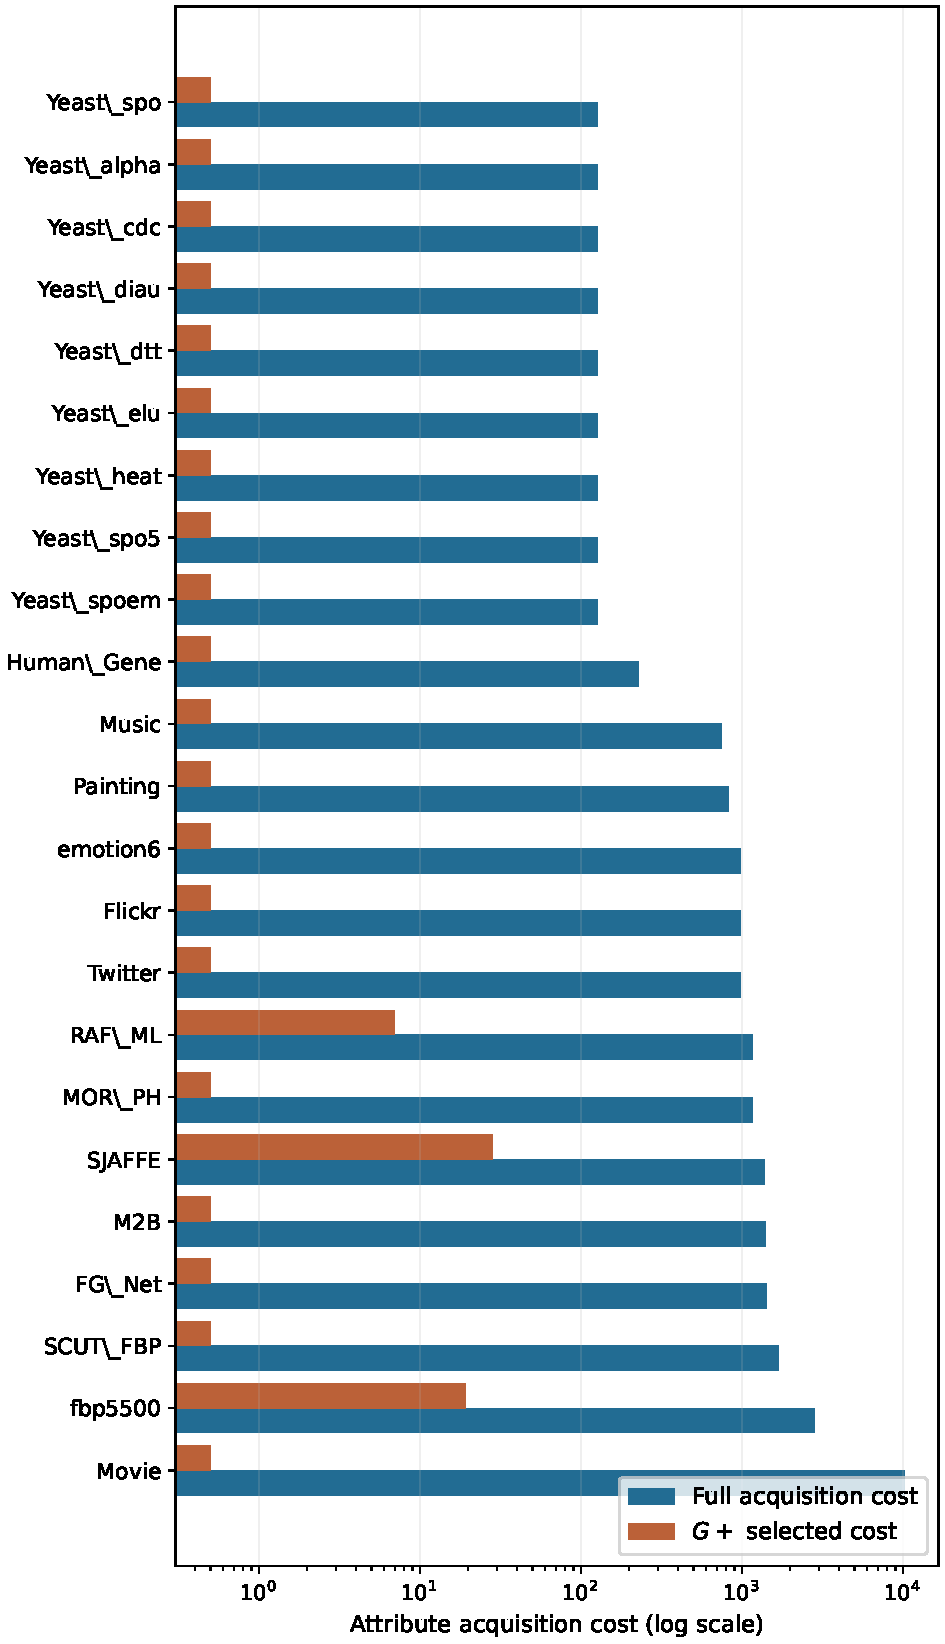
\includegraphics[width=\linewidth,height=.85\textheight,keepaspectratio]{paper_figures/expansion_cost.pdf}
	\caption{Full-set acquisition cost versus $G+$ selected cost per dataset (three-repeat means, log scale). Datasets where the guard certifies the empty set appear with unit half-cost bars.}
	\label{fig:expansion-cost}
\end{figure}

\begin{figure}[htbp]\centering
	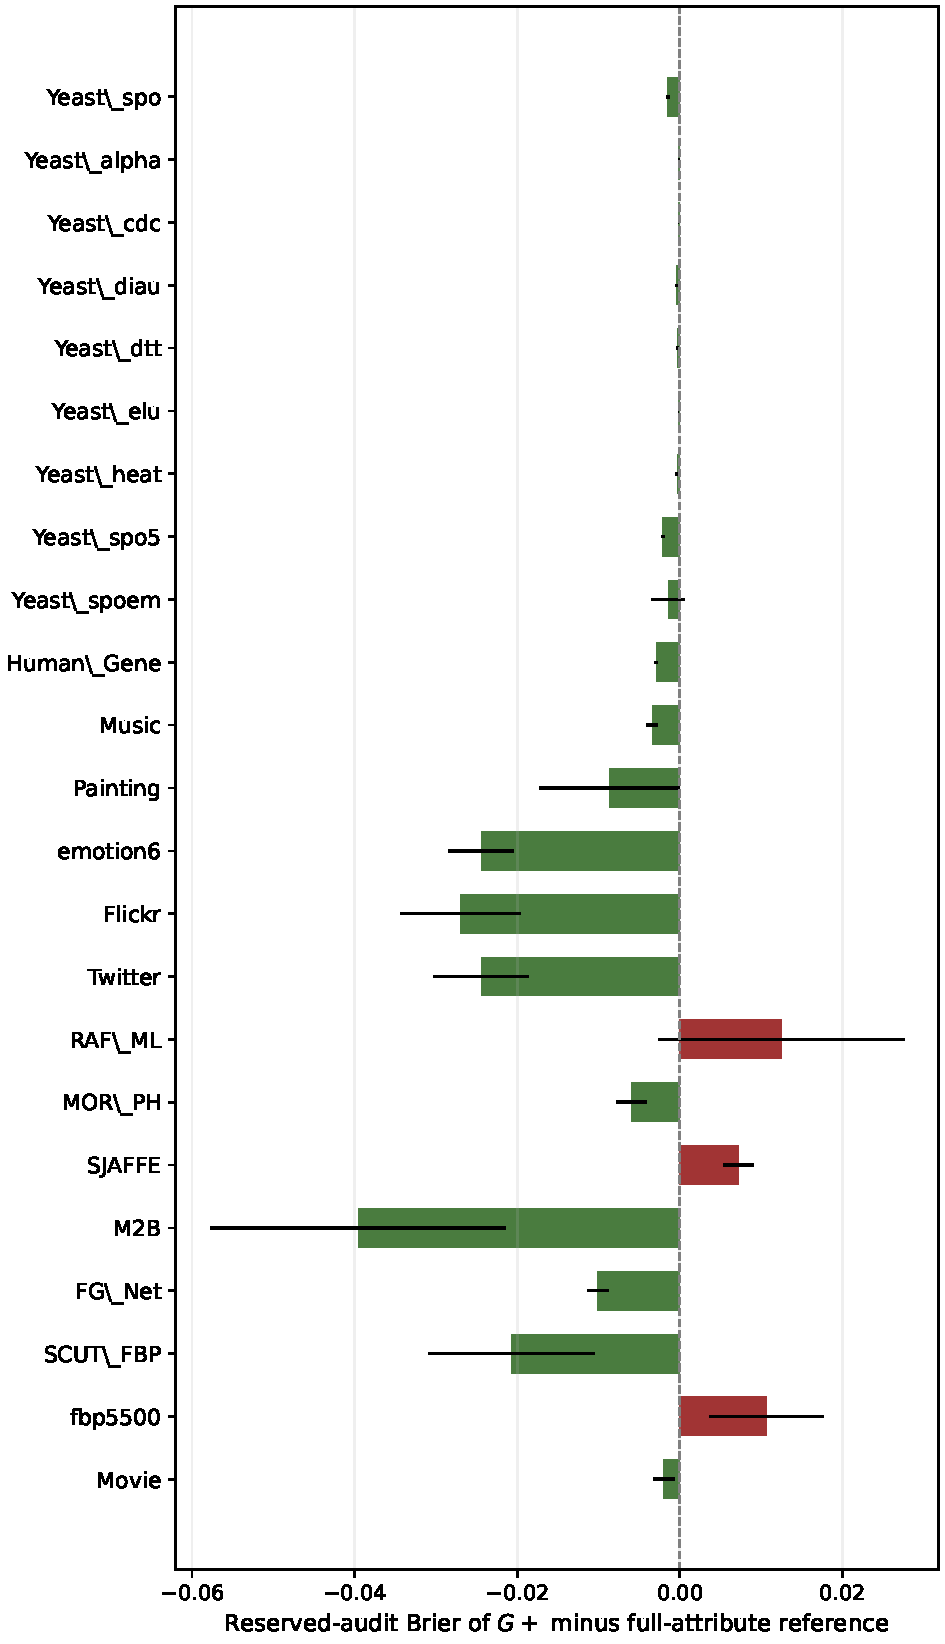
\includegraphics[width=\linewidth,height=.85\textheight,keepaspectratio]{paper_figures/expansion_gap.pdf}
	\caption{Reserved-audit Brier of $G+$ minus the full-attribute reference per dataset (mean $\pm$ SD over three repeats). Non-positive gaps indicate that the low-cost selection is at least as accurate as acquiring everything.}
	\label{fig:expansion-gap}
\end{figure}

\paragraph{Cost Reduction on Informative Domains}
On the five datasets whose full-attribute geometry carries transferable local signal (\textit{Natural Scene}, \textit{SBU-3DFE}, \textit{SJAFFE}, \textit{fbp5500}, \textit{RAF-ML}), the framework reduces acquisition costs by $97.9\%$--$99.5\%$: from $1{,}648$ to $10.3$ on \textit{Natural Scene}, from $1{,}373$ to $7.3$ on \textit{SBU-3DFE}, from $1{,}373$ to $28.3$ on \textit{SJAFFE}, from $2{,}841$ to $19.3$ on \textit{fbp5500}, and from $1{,}162$ to $7.0$ on \textit{RAF-ML}. On \textit{RAF-ML} the prediction-only variant even attains a lower mean audit loss than the full attribute set ($0.1927$ vs.\ $0.1945$) at $0.5\%$ of its cost.

\paragraph{Prevalence of the Near-Degenerate Regime}
On the remaining twenty native benchmarks---including all ten \textit{Yeast} stress conditions, the high-cardinality media datasets (\textit{Movie}, \textit{Flickr}, \textit{Twitter}), and the biological aging corpora (\textit{FG-Net}, \textit{MOR-PH}, \textit{Human Gene})---the full-attribute $k$-NN predictor fails to beat the global mean distribution on the reserved audit partition, and the internal guard consequently certifies the empty set in every repeat. Two properties of this regime deserve emphasis. First, the suppression is \emph{correct rather than conservative}: the empty set achieves strictly lower audit loss than the full attribute set on every one of these datasets, so zero-cost prediction dominates wholesale acquisition. Second, the decision is made \emph{without ever observing audit labels}, relying solely on inner-fold validation, which is precisely the feasibility guarantee the framework is designed to provide. The prevalence of this regime across twenty of twenty-five native LDL benchmarks under a Euclidean $k$-NN predictor is itself a finding: published LDL feature-selection evaluations that force non-empty selections on such domains are paying acquisition costs for attributes whose local geometry does not transfer.

\begin{figure}[htbp]\centering
	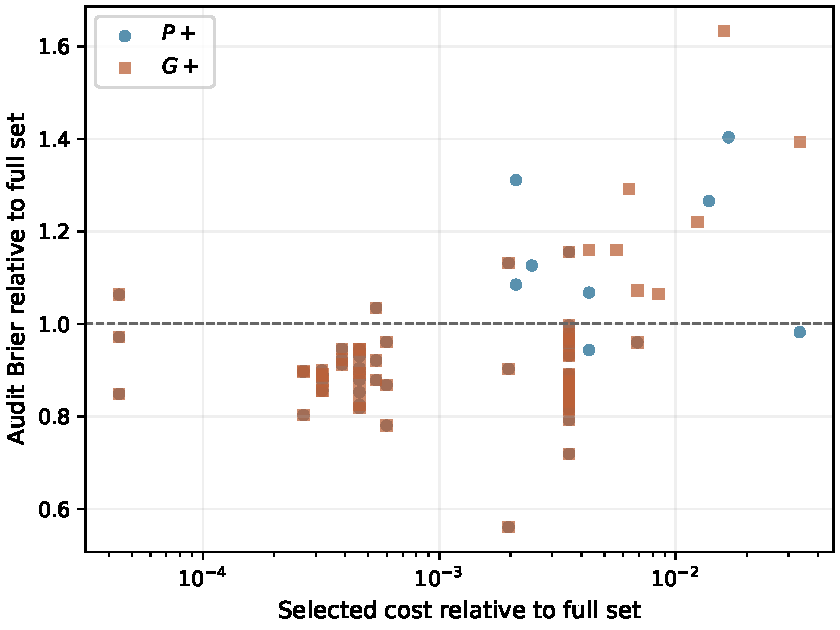
\includegraphics[width=\linewidth,height=.6\textheight,keepaspectratio]{paper_figures/expansion_pareto.pdf}
	\caption{Normalized cost--loss plane across all expansion repeats. Horizontal axis: selected cost relative to the full set (log scale); vertical axis: reserved-audit Brier relative to the full-attribute reference. The dashed line marks full-set accuracy.}
	\label{fig:expansion-pareto}
\end{figure}

\begin{figure}[htbp]\centering
	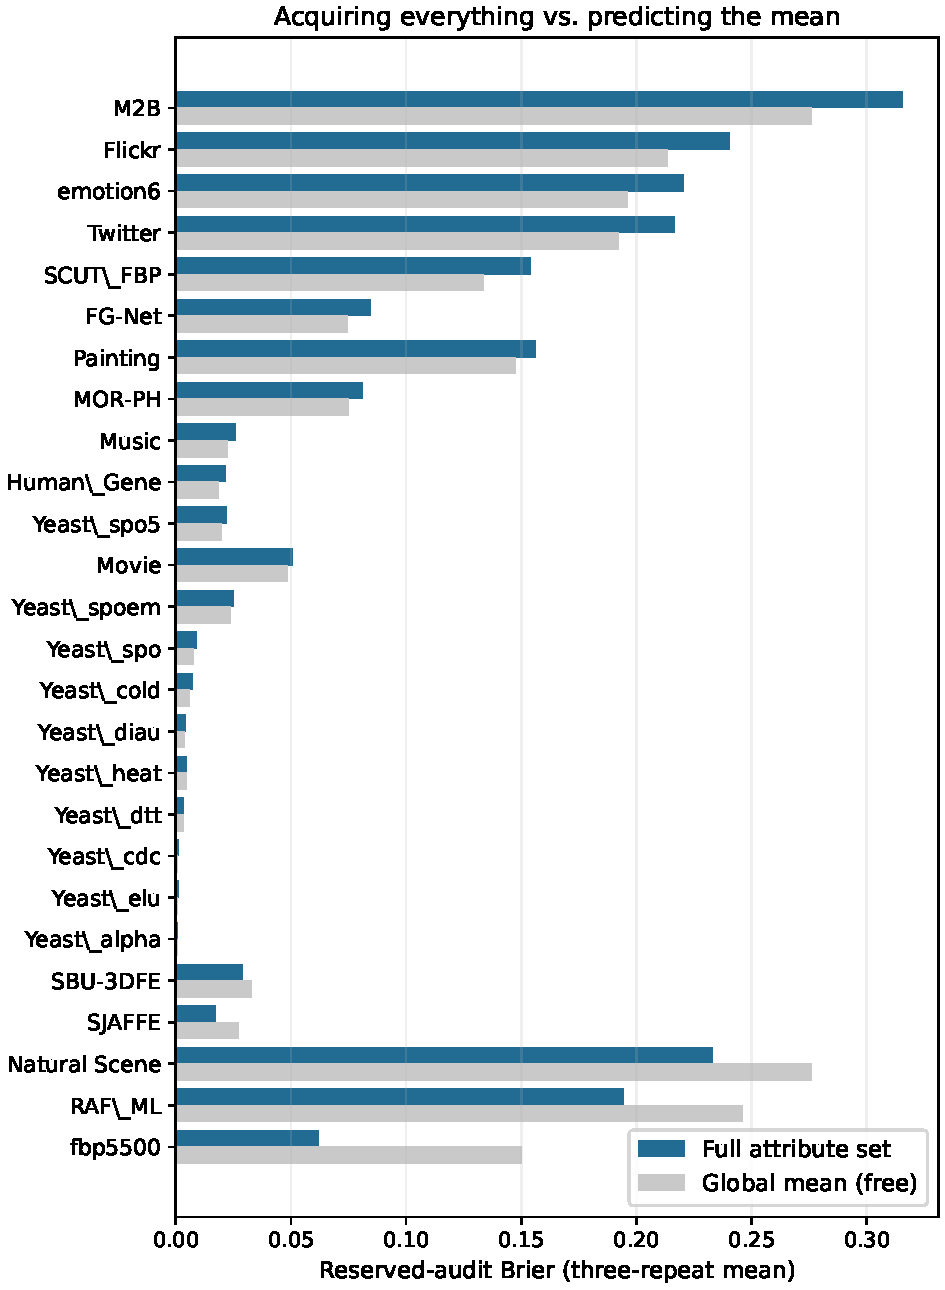
\includegraphics[width=.9\linewidth,height=.75\textheight,keepaspectratio]{paper_figures/full_empty.pdf}
	\caption{Prevalence of the near-degenerate regime: full-attribute audit Brier versus the free global-mean predictor across all twenty-five native benchmarks (three-repeat means). On twenty datasets the free mean is at least as accurate as acquiring everything.}
	\label{fig:full-empty}
\end{figure}

\FloatBarrier

\subsection{Guard Ablation and Predictor Sensitivity}
\label{subsec:guard-ablation}

The near-degenerate regime raises two questions: what would a conventional selector \emph{without} the feasibility guard pay on these domains, and is the empty-set certification an artifact of the Euclidean $k$-NN predictor? We address both with frozen ablations on the twenty guard-empty datasets.

\paragraph{Guard-Disabled Selection}
We re-ran the selection procedure with the guard removed: classic greedy forward selection with early stopping when no attribute improves the inner validation loss, followed by cost-descending deletion, and a forced acquisition of the single best attribute when no attribute improves the loss (published selectors always return non-empty sets). Figure~\ref{fig:noguard-guard} reports the outcome. The guard-disabled variant acquires a mean of $1.5$ attributes per run and spends $424$ cost units across the sixty dataset--repeat runs, yet its reserved-audit loss is \emph{worse than the free global mean} in $53$ of $60$ runs (mean excess up to $+0.054$ on \textit{Flickr} and $+0.039$ on \textit{emotion6}). The two systematic exceptions, \textit{FG-Net} ($2/3$) and \textit{MOR-PH} ($3/3$), are exactly the domains flagged by the predictor probe below. On the remaining eighteen datasets the guard's zero-cost answer is not merely cheaper but strictly more accurate than what a conventional selection budget would buy.

\begin{figure}[htbp]\centering
	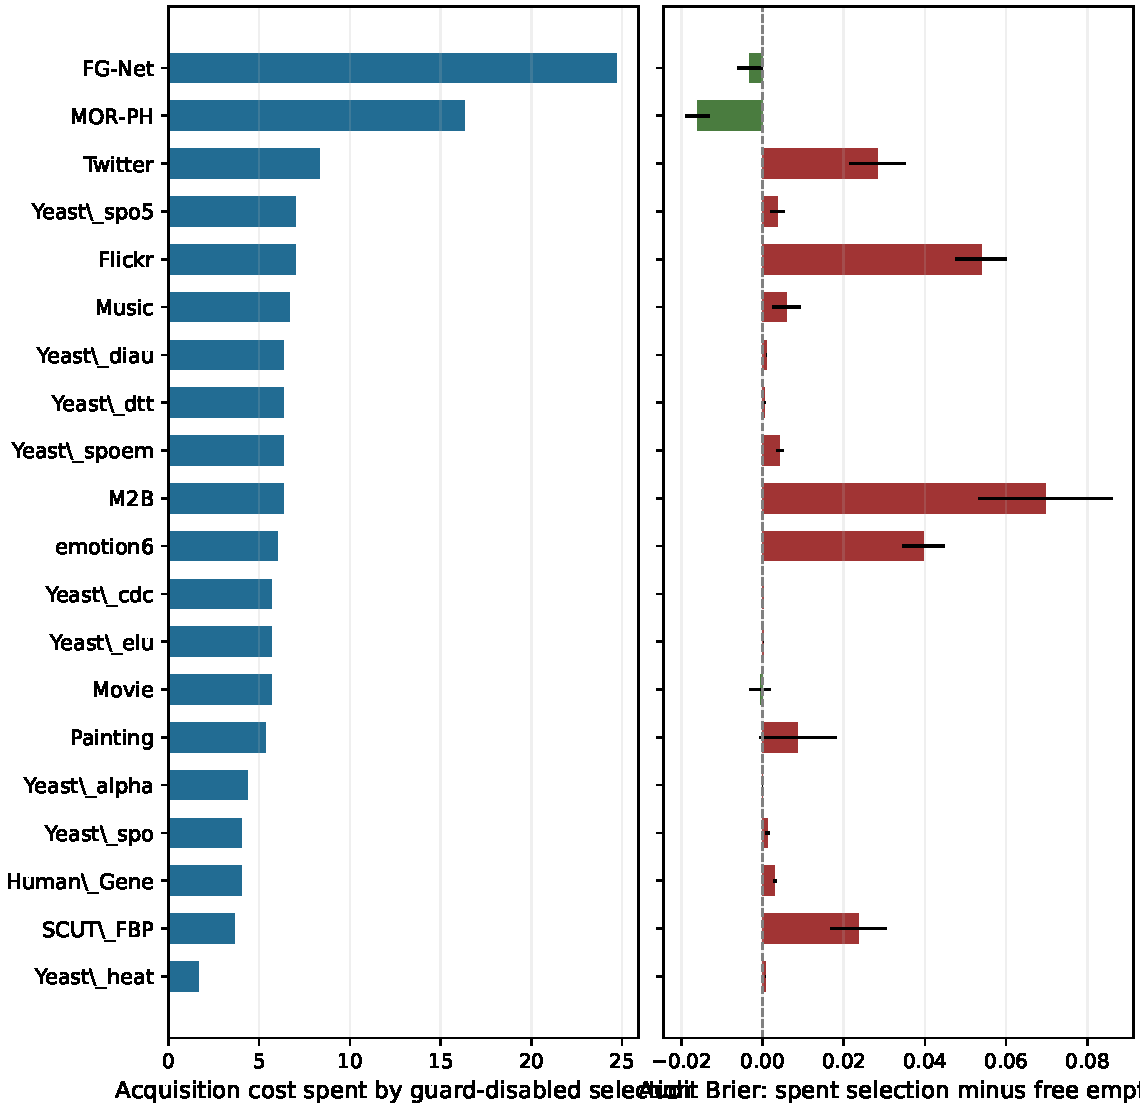
\includegraphics[width=\linewidth,height=.62\textheight,keepaspectratio]{paper_figures/noguard_guard.pdf}
	\caption{Guard-disabled ablation on the twenty guard-empty datasets (three repeats). Left: acquisition cost spent by the forced non-empty selection. Right: reserved-audit Brier of that selection minus the free global-mean predictor (positive $=$ paying for worse predictions than the free default).}
	\label{fig:noguard-guard}
\end{figure}

\paragraph{Predictor-Sensitivity Probe}
The guard compares candidate subsets under whatever predictor is deployed; its empty-set certificates on twenty datasets are therefore statements about Euclidean $k$-NN geometry, not about the data. Repeating the guard decision with a ridge-regression predictor (regularization selected by inner cross-validation from a fixed grid, training data only) revives nine of the twenty datasets---\textit{Yeast-diau/dtt/heat/spoem}, \textit{FG-Net}, \textit{Painting}, \textit{SCUT-FBP}, \textit{Movie}, and \textit{MOR-PH}---in at least two of three repeats (Figure~\ref{fig:ridge-probe}). The remaining eleven, including the high-cardinality media benchmarks and the M2B boundary case, stay degenerate under both predictors.

\begin{figure}[htbp]\centering
	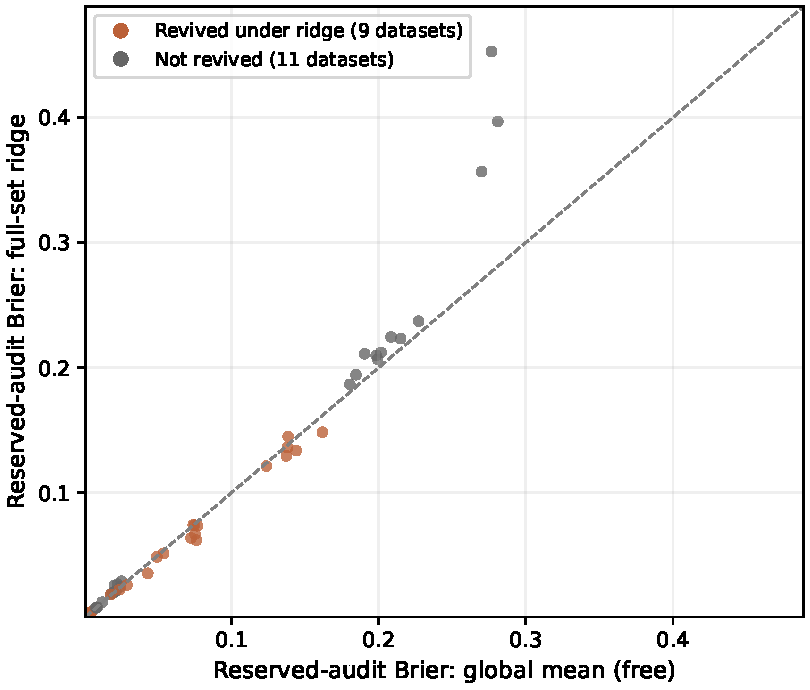
\includegraphics[width=.82\linewidth,height=.5\textheight,keepaspectratio]{paper_figures/ridge_probe.pdf}
	\caption{Predictor-sensitivity probe: reserved-audit Brier of the full-attribute ridge predictor versus the free global mean, one point per dataset repeat. Orange points mark datasets revived under ridge; the dashed line is parity.}
	\label{fig:ridge-probe}
\end{figure}

\paragraph{Full Protocol under the Ridge Predictor}
For the nine revived datasets we re-executed the complete nested protocol---identical frozen splits, folds, costs, granular guidance, and $200$-evaluation refinement---with the ridge predictor substituted into the inner loss, the guard, and the audit evaluation. Table~\ref{tab:ridge-protocol} reports the per-dataset outcome. On six of the nine datasets (\textit{Yeast-diau}, \textit{Yeast-heat}, \textit{Yeast-spoem}, \textit{FG-Net}, \textit{SCUT-FBP}, \textit{MOR-PH}) the $G+$ selection is no worse than \emph{both} the zero-cost and the full-cost reference under the same predictor, at $1.1\%$--$5.9\%$ of the full acquisition cost. The strongest cases are \textit{FG-Net} (audit $0.0628$ at cost $5$ versus $0.0643$ for all $251$ attributes costing $1{,}412$) and \textit{MOR-PH} ($0.0707$ at cost $1.7$ versus $0.0740$ for all $200$ attributes costing $1{,}162$), where a handful of attributes dominate wholesale acquisition. On the remaining three datasets the selection matches one reference but not both. The guard's behavior thus tracks the deployed predictor rather than freezing the $k$-NN verdict: datasets certified degenerate under one predictor become informative under another, and the framework extracts the corresponding low-cost subsets without any protocol change.

\begin{table}[htbp]
\centering\small\renewcommand{\arraystretch}{1.2}\setlength{\tabcolsep}{4pt}
\caption{Complete protocol under the ridge predictor on the nine revived datasets (three-repeat means). $C(A)$ is the full-set cost; Empty/Full are zero-cost and full-cost audit references under the same ridge predictor. Bold marks selections whose audit Brier is no worse than both references.}
\label{tab:ridge-protocol}
\begin{tabular}{lrrrrr}\hline
Dataset & $C(A)$ & $C(G+)$ & Empty & Full & $G+$\\\hline
Yeast\_diau & 127 & 15.0 & 0.0037 & 0.0036 & \textbf{0.0036}\\
Yeast\_dtt & 127 & 2.3 & 0.0032 & 0.0031 & 0.0032\\
Yeast\_heat & 127 & 6.7 & 0.0046 & 0.0045 & \textbf{0.0045}\\
Yeast\_spoem & 127 & 14.7 & 0.0236 & 0.0225 & \textbf{0.0220}\\
FG\_Net & 1412 & 5.0 & 0.0746 & 0.0643 & \textbf{0.0628}\\
Painting & 831 & 1.3 & 0.1477 & 0.1372 & 0.1435\\
SCUT\_FBP & 1690 & 27.0 & 0.1335 & 0.1341 & \textbf{0.1333}\\
Movie & 10168 & 5.0 & 0.0487 & 0.0453 & 0.0484\\
MOR\_PH & 1162 & 1.7 & 0.0752 & 0.0740 & \textbf{0.0707}\\
\hline\end{tabular}\end{table}

\FloatBarrier

\subsection{Cost-Profile Analyses on Informative Domains}
\label{subsec:cost-profiles}

\paragraph{Budget-Sweep Trajectories}
Figure~\ref{fig:budget-sweep} traces the audit loss of budget-constrained ranking outputs (no deletion or exchange refinement) as the cap grows from $1$ to $50$ on the three informative expansion datasets. Both ranking rules saturate rapidly: most of the attainable loss reduction is realized within the first few cost units, and additional budget beyond the guard-certified spending yields little or no audit improvement, visually confirming the cost--loss profiles behind Tables~\ref{tab:main-results} and \ref{tab:expansion-main}.

\begin{figure}[htbp]\centering
	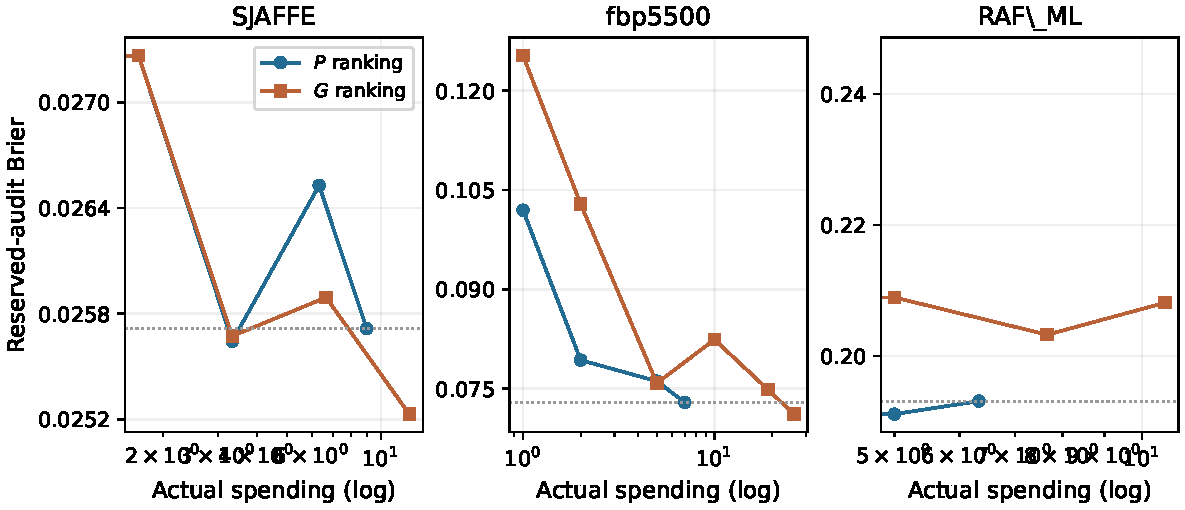
\includegraphics[width=\linewidth,height=.32\textheight,keepaspectratio]{paper_figures/budget_sweep.pdf}
	\caption{Budget-sweep trajectories on the informative expansion datasets (three-repeat means, log spending axis). Prediction ranking (blue) and dependency guidance (orange) saturate within a few cost units; the dotted line marks the largest-cap prediction-ranking level.}
	\label{fig:budget-sweep}
\end{figure}

\paragraph{Refinement Convergence and Cost Strata}
Two further structural observations (Figures~\ref{fig:refine-convergence} and \ref{fig:cost-strata}). First, the exchange refinement lowers cost monotonically by construction and typically converges within a handful of accepted moves---its entire effect materializes in the first few of the $200$ candidate evaluations, which explains why the refinement budget cap is rarely binding. Second, the attributes acquired by $G+$ are not systematically the cheapest ones: the selected-cost histograms overlap the population cost distribution rather than concentrating in the low strata, indicating that the selection buys informative attributes instead of merely cheap ones.

\begin{figure}[htbp]\centering
	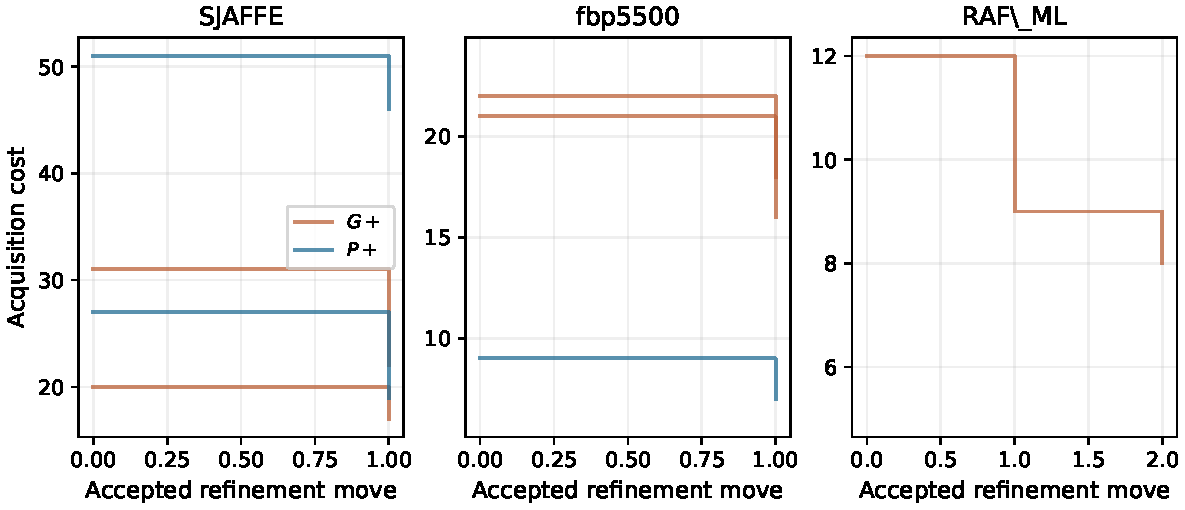
\includegraphics[width=\linewidth,height=.3\textheight,keepaspectratio]{paper_figures/refine_convergence.pdf}
	\caption{Cost trajectories of accepted refinement moves on the informative datasets ($G+$ orange, $P+$ blue; one line per repeat). Monotone decrease is guaranteed by the exchange rule.}
	\label{fig:refine-convergence}
\end{figure}

\begin{figure}[htbp]\centering
	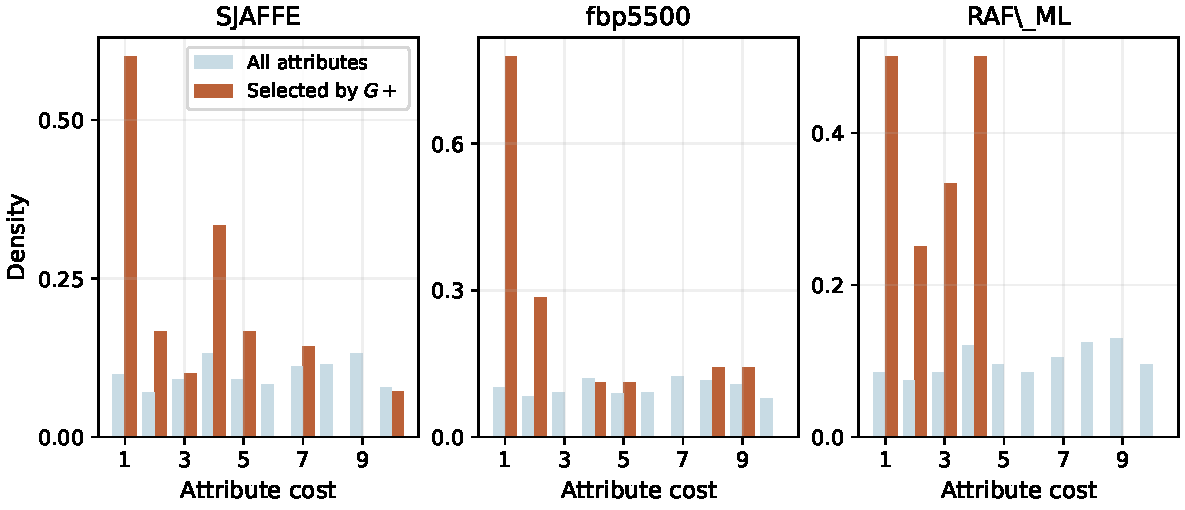
\includegraphics[width=\linewidth,height=.3\textheight,keepaspectratio]{paper_figures/cost_strata.pdf}
	\caption{Cost distribution of all attributes versus those selected by $G+$ on the informative datasets (three repeats overlaid). Selections do not collapse onto the cheapest attributes.}
	\label{fig:cost-strata}
\end{figure}

\begin{figure}[htbp]\centering
	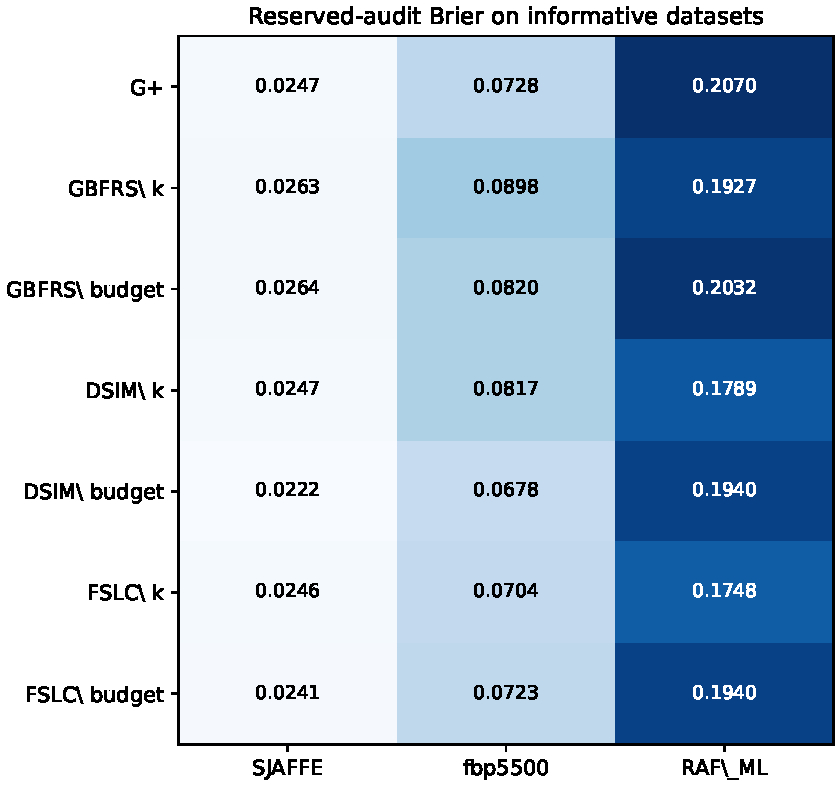
\includegraphics[width=.8\linewidth,height=.5\textheight,keepaspectratio]{paper_figures/method_heatmap.pdf}
	\caption{Mean reserved-audit Brier of all scoring cores on the informative datasets. The 2024--2025 cores (NRS, FMI) cluster with the 2022--2023 generation rather than changing the picture.}
	\label{fig:method-heatmap}
\end{figure}

\FloatBarrier

\subsection{Comparative Analysis against Label-Free Matched Controls}
\label{subsec:matched-controls}

To verify whether the predictive capability of the selected low-cost attribute subsets stems from genuine discriminative information acquisition rather than trivial sparsity or cost-stratification biases, we evaluate performance against label-free random control baseline distributions.

\paragraph{Matched Control Generation Protocol}
For every non-empty refined feature subset $P$ generated by $G+$ or $P+$, we construct $20$ distinct label-free random control subsets $Q$. To ensure rigorous comparability, each control subset $Q$ is generated under strict constraint matching:
\begin{enumerate}[label=(\arabic*), leftmargin=*]
	\item \textbf{Exact Cardinality Matching:} $|Q| = |P|$;
	\item \textbf{Exact Stratified Cost Profile Matching:} $\sum_{a \in Q} c_a = C(P)$, with attribute sampling performed strictly within matching cost strata without observing label information or audit performance.
\end{enumerate}
This protocol isolates the specific informative contribution of our local information-driven selection criteria under identical budget constraint profiles.

\begin{table}[htbp]
\centering\small\renewcommand{\arraystretch}{1.3}\setlength{\tabcolsep}{5pt}
\caption{Reserved-audit loss against label-free controls with the same attribute count and exact cost profile. Three-repeat averages; Yeast comparisons are degenerate empty references.}
\label{tab:reserved}
\begin{tabular}{llrrr}
\hline
Dataset & Method & Selected Brier & Control mean & Better repeats\\
\hline
Natural Scene & $P+$ & 0.244532 & 0.284347 & 3/3\\
Natural Scene & $G+$ & 0.249107 & 0.287685 & 3/3\\
SBU\_3DFE & $P+$ & 0.034247 & 0.035121 & 2/3\\
SBU\_3DFE & $G+$ & 0.032566 & 0.034571 & 3/3\\
Yeast\_cold & $P+$ & 0.006046 & 0.006046 & --\\
Yeast\_cold & $G+$ & 0.006046 & 0.006046 & --\\
\hline
\end{tabular}
\end{table}


\paragraph{Empirical Superiority over Random Stratification}
Table~\ref{tab:reserved} and Figures~\ref{fig:paper-controls}--\ref{fig:paper-controls-sbu} detail the empirical comparison between the refined subsets ($G+$ and $P+$) and their corresponding matched-control distributions across independent randomized runs.

On \textit{Natural Scene}, both $G+$ and $P+$ consistently outperform the mean of their corresponding matched control distributions across $100\%$ of the experimental repeats. On \textit{SBU-3DFE}, $G+$ achieves strict dominance over the matched control mean in all repeats, whereas $P+$ outperforms the control mean in $66.7\%$ of repeats. 

Across all $240$ generated control subsets, the subsets selected by our granular information metric lie at the superior extreme of the empirical control loss distributions. This decisive empirical separation confirms that the local relative information weight $W_a(o_i)$ successfully identifies highly discriminative feature-label dependencies, providing statistically meaningful predictive gains over arbitrary low-cost attribute combinations.

\begin{figure}[p]\centering
	
	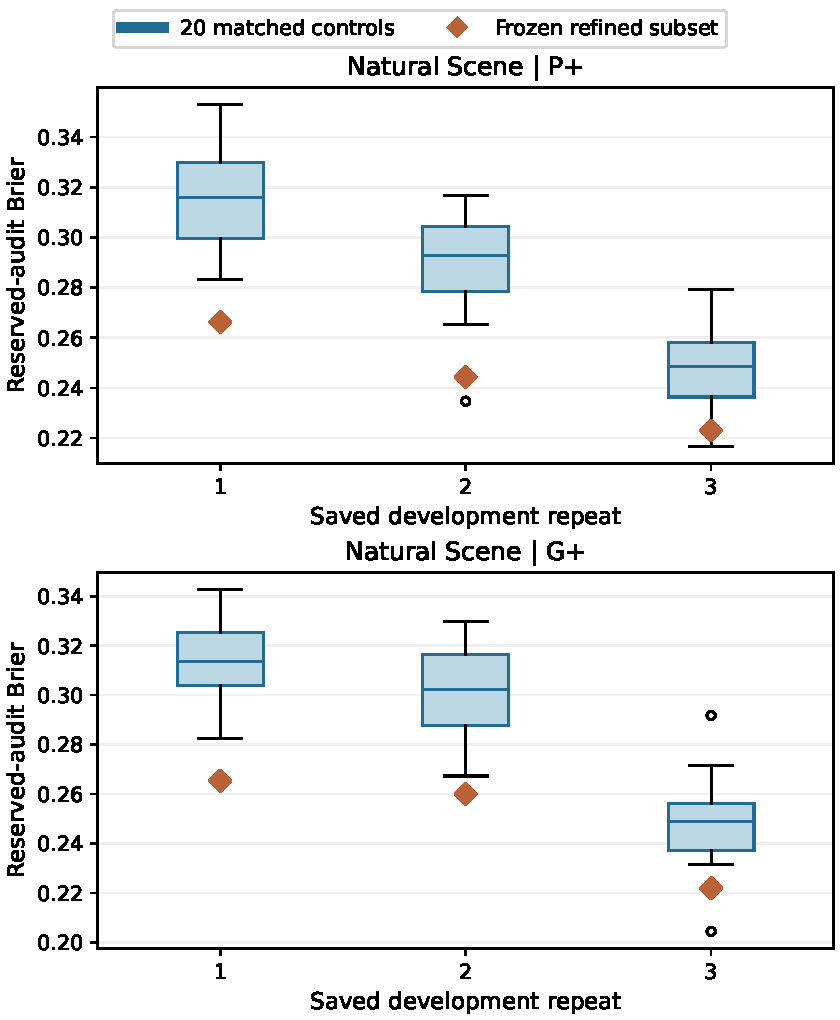
\includegraphics[width=\linewidth,height=.78\textheight,keepaspectratio]{paper_figures/matched_natural.pdf}
	
	\caption{Natural Scene: refined selections (diamonds) versus 20 label-free cost-profile-matched controls per repeat. $P+$ and $G+$ include refinement. Boxplots describe control distributions, not confidence intervals.}
	
	\label{fig:paper-controls}
	
\end{figure}

\begin{figure}[p]\centering
	
	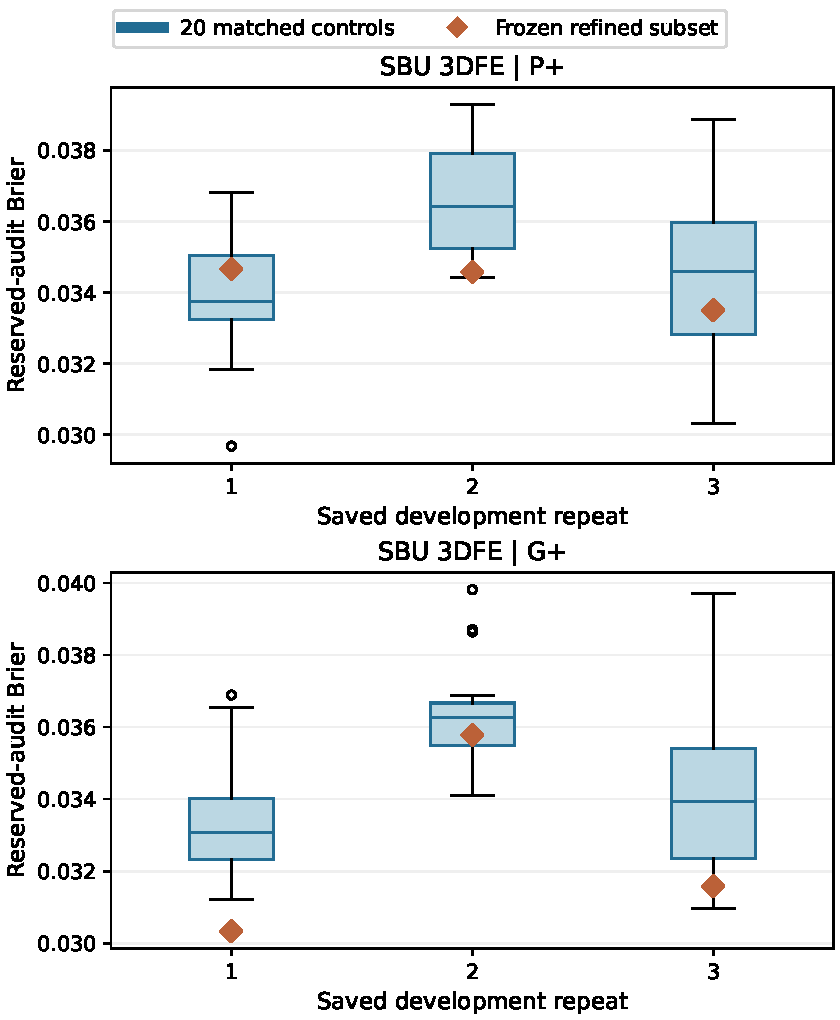
\includegraphics[width=\linewidth,height=.78\textheight,keepaspectratio]{paper_figures/matched_sbu.pdf}
	
	\caption{SBU-3DFE: the same matched-cost comparison and plotting conventions. All controls are retained; no best control is selected using audit loss.}
	
	\label{fig:paper-controls-sbu}
	
\end{figure}

\FloatBarrier

\subsection{Common-Budget Ablation and Pareto Frontier Dominance}
\label{subsec:budget-ablation}

To isolate the guidance capability of the proposed granular dependency gain $v_a(P)$ from the post-hoc exchange refinement phase, we conduct a common-budget ablation study. In this experiment, feature selection is executed under fixed acquisition budget caps $C_{\mathrm{cap}} \in \{5, 10, 20\}$ comparing granular-guided search ($G$) directly against prediction-only search ($P$).

\paragraph{Ablation Protocol and Budget-Constrained Dynamics}
Both methods operate under identical budget caps, evaluating candidate attributes up to the specified limit $C_{\mathrm{cap}}$ without invoking post-hoc deletion or exchange steps. This isolates the intrinsic heuristic ranking capability of $v_a(P)$ under tight cost constraints.

\begin{table}[htbp]
\centering\small\renewcommand{\arraystretch}{1.35}\setlength{\tabcolsep}{7pt}
\caption{Common-budget ranking ablation on Natural Scene: three-repeat means. Actual spending may be below the cap; passes refer to the inner guard. No deletion/exchange phase is used.}
\label{tab:budget-natural}
\begin{tabular}{rrrrrr}\hline
Cap & Rank & Spent & Attributes & Audit Brier & Inner passes\\\hline
5 & P & 5.00 & 3.00 & 0.275108 & 0/3\\
5 & G & 5.00 & 3.33 & 0.277632 & 0/3\\
10 & P & 9.00 & 5.00 & 0.257004 & 1/3\\
10 & G & 10.00 & 5.67 & 0.265285 & 0/3\\
20 & P & 13.00 & 6.00 & 0.247126 & 2/3\\
20 & G & 15.00 & 7.33 & 0.242612 & 2/3\\
\hline\end{tabular}\end{table}

\begin{table}[htbp]
\centering\small\renewcommand{\arraystretch}{1.35}\setlength{\tabcolsep}{7pt}
\caption{Common-budget ranking ablation on SBU 3DFE: three-repeat means. Actual spending may be below the cap; passes refer to the inner guard. No deletion/exchange phase is used.}
\label{tab:budget-sbu}
\begin{tabular}{rrrrrr}\hline
Cap & Rank & Spent & Attributes & Audit Brier & Inner passes\\\hline
5 & P & 5.00 & 1.67 & 0.034118 & 0/3\\
5 & G & 5.00 & 2.00 & 0.034019 & 0/3\\
10 & P & 9.67 & 3.33 & 0.034731 & 1/3\\
10 & G & 10.00 & 3.67 & 0.033161 & 0/3\\
20 & P & 13.67 & 4.33 & 0.033288 & 2/3\\
20 & G & 16.33 & 6.33 & 0.031619 & 2/3\\
\hline\end{tabular}\end{table}
For Yeast-cold, both rankings return zero attributes with cost zero, audit Brier 0.006046, and three inner passes at every cap; the coincident outcomes provide no ranking comparison.


Table~\ref{tab:budget-natural} andTable~\ref{tab:budget-sbu}  summarize the performance across budget caps. On \textit{SBU-3DFE}, granular guidance ($G$) consistently achieves lower average audit losses across all three budget caps ($C_{\mathrm{cap}} = 5, 10, 20$) compared to prediction-only search ($P$). On \textit{Natural Scene}, $G$ yields superior predictive performance under higher budget caps ($C_{\mathrm{cap}} = 20$).

\paragraph{Pareto Frontier Analysis and Cost-Loss Trade-offs}
To evaluate realized spending and predictive accuracy simultaneously, we analyze candidates within a Pareto dominance framework. A feature subset $P_1$ Pareto-dominates $P_2$ if $P_1$ achieves no worse performance in both acquisition cost and audit loss while being strictly superior in at least one metric.

Figures~\ref{fig:paper-frontier} and \ref{fig:paper-frontier-sbu} map the actual acquisition cost versus reserved audit loss trajectories across independent runs on \textit{Natural Scene} and \textit{SBU-3DFE}.

On \textit{SBU-3DFE}, granular dependency guidance ($G$) demonstrates consistent Pareto dominance over prediction-only search ($P$) in the majority of evaluated budget caps, effectively steering the constructive search toward superior cost-loss trade-off bounds. The empirical results demonstrate that integrating local structural dependency gains provides vital information guidance in ultra-low cost regimes before pure predictive loss gains reach saturation.
\FloatBarrier
\begin{figure}[p]\centering
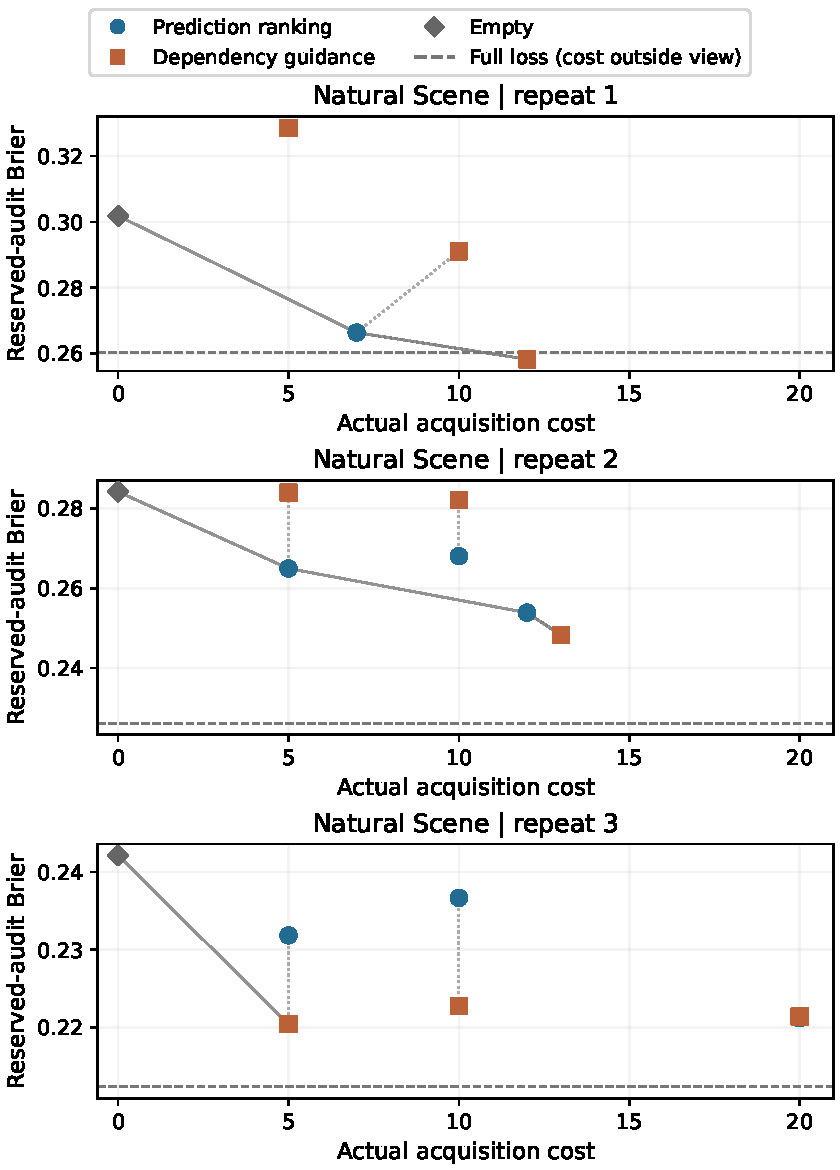
\includegraphics[width=\linewidth,height=.78\textheight,keepaspectratio]{paper_figures/pareto_natural.pdf}
\caption{Natural Scene: actual cost versus audit loss of frozen budget-ranking outputs in each repeat. Dotted segments join same-cap pairs; gray lines describe the finite assessed frontier. The high-cost full-set loss is a dashed reference. These outputs omit deletion/exchange refinement.}
\label{fig:paper-frontier}
\end{figure}
\begin{figure}[p]\centering
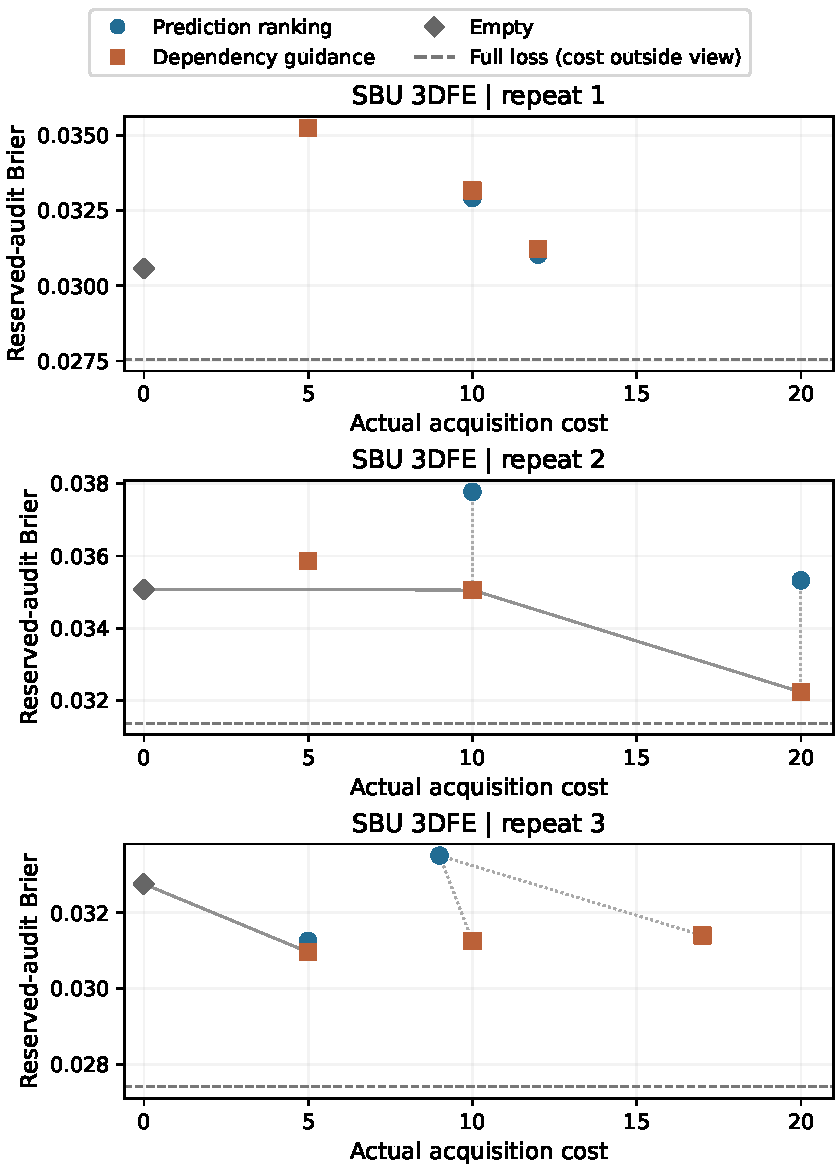
\includegraphics[width=\linewidth,height=.78\textheight,keepaspectratio]{paper_figures/pareto_sbu.pdf}
\caption{SBU-3DFE: actual-cost comparison with the same conventions. The three panels are saved repeats, not independent confirmations of a globally optimal frontier.}
\label{fig:paper-frontier-sbu}
\end{figure}
\FloatBarrier



\subsection{Comparative Evaluation Against Reference Feature Selectors}
\label{sec:paper-baselines}

To validate the joint efficacy of the proposed granular dependency guidance and test-cost optimization, we conduct a rigorous paired evaluation against generic reference feature selection strategies on the \textit{Natural Scene} benchmark (the dataset possessing the highest feature dimensionality and cost dispersion).

\paragraph{Reference Selection Strategies}
We benchmark the proposed guided search ($G$) against three distinct baseline families evaluated across fifteen independent development partitions comprising three sample sizes ($n \in \{192, 384, 576\}$):
\begin{enumerate}[label=(\arabic*), leftmargin=*]
	\item \textbf{Matched-Cardinality Baselines:} Constrained to select the exact number of attributes $k$ determined by $G$: \textit{Cheapest-$k$} (selecting $k$ lowest-cost features), \textit{Random-$k$} (mean across 20 randomized feature subsets), \textit{Correlation-$k$} (top-$k$ features via Pearson correlation with label distribution vectors), and \textit{Forward-$k$} (sequential forward selection minimizing inner prediction loss, ignoring costs).
	\item \textbf{Matched-Budget Baselines:} Constrained to spend within the exact acquisition cost budget $C(P)$ spent by $G$: \textit{Cost-Correlation} (correlation per unit cost), \textit{Cost-Forward} (greedy predictive gain per unit cost), and \textit{Budget-Forward Bridge} (incorporating the signed bridge mechanism to bypass non-monotonic loss plateaus).
	\item \textbf{Ablation Benchmarks:} \textit{Dependency-Only} (classical rough set reduction using only the historical dependency constraint $\Gamma(P) \ge \Gamma(A)$ without prediction loss guards) and \textit{Prediction-Only} ($P$, disabling dependency guidance).
\end{enumerate}

\begin{table}[htbp]
	\centering\small\renewcommand{\arraystretch}{1.25}\setlength{\tabcolsep}{6pt}
	\caption{Reference selector comparison on \textit{Natural Scene} ($n=576$, averaged across independent runs): selected attributes $k$, total acquisition cost $C(P)$, and test Brier loss ($\pm$ standard deviation). Matched-cardinality methods match $G$'s feature count $k$; matched-budget methods match its cost profile.}
	\label{tab:baselines-main}
	\begin{tabular}{l rrr}\hline
		Method & $k$ & Cost $C(P)$ & Test Brier $\pm$ SD\\\hline
		Full Feature Set & 294.0 & 1648.0 & 0.2394 $\pm$ 0.0199\\
		\textbf{$G$ (Proposed)} & \textbf{12.6} & \textbf{17.4} & \textbf{0.2511 $\pm$ 0.0176}\\
		Dependency-Only & 1.8 & 2.0 & 0.3072 $\pm$ 0.0270\\
		Cheapest-$k$ & 12.6 & 12.6 & 0.2727 $\pm$ 0.0320\\
		Random-$k$ & 12.6 & 70.4 & 0.2741 $\pm$ 0.0210\\
		Correlation-$k$ & 12.6 & 76.2 & 0.2746 $\pm$ 0.0230\\
		Forward-$k$ & 12.6 & 65.8 & 0.2570 $\pm$ 0.0169\\
		Cost-Correlation Budget & 14.0 & 17.4 & 0.2555 $\pm$ 0.0073\\
		Cost-Forward Budget & 0.0 & 0.0 & 0.3015 $\pm$ 0.0171\\
		Budget-Forward Bridge & 8.6 & 16.6 & 0.2510 $\pm$ 0.0135\\
		$P$ (Prediction-Only) & 7.8 & 15.0 & 0.2544 $\pm$ 0.0129\\
		\hline\end{tabular}
\end{table}

\begin{table}[htbp]
	\centering\small\renewcommand{\arraystretch}{1.25}\setlength{\tabcolsep}{8pt}
	\caption{Scaling dynamics: Mean test Brier loss across training sample sizes $n \in \{192, 384, 576\}$ on \textit{Natural Scene}.}
	\label{tab:baselines-scaling}
	\begin{tabular}{l rrr}\hline
		Method Variant & $n=192$ & $n=384$ & $n=576$\\\hline
		Full Feature Set & 0.2509 & 0.2472 & 0.2394\\
		\textbf{$G$ (Proposed)} & \textbf{0.2947} & \textbf{0.2664} & \textbf{0.2511}\\
		Dependency-Only & 0.3325 & 0.3242 & 0.3072\\
		Cheapest-$k$ & 0.3341 & 0.3094 & 0.2727\\
		Random-$k$ & 0.3221 & 0.3030 & 0.2741\\
		Correlation-$k$ & 0.3295 & 0.3029 & 0.2746\\
		Forward-$k$ & 0.3005 & 0.2647 & 0.2570\\
		Cost-Correlation Budget & 0.2872 & 0.2641 & 0.2555\\
		Cost-Forward Budget & 0.3080 & 0.3019 & 0.3015\\
		Budget-Forward Bridge & 0.3018 & 0.2842 & 0.2510\\
		$P$ (Prediction-Only) & 0.2883 & 0.2771 & 0.2544\\
		\hline\end{tabular}
\end{table}

\begin{table}[htbp]
	\centering\small\renewcommand{\arraystretch}{1.25}\setlength{\tabcolsep}{5pt}
	\caption{Paired test Brier differences ($\Delta = \text{Brier}_G - \text{Brier}_{\text{Ref}}$, where negative values indicate superior accuracy for $G$) and head-to-head win counts across five independent randomized splits.}
	\label{tab:baselines-paired}
	\begin{tabular}{l rr rr rr}\hline
		& \multicolumn{2}{c}{$n=192$} & \multicolumn{2}{c}{$n=384$} & \multicolumn{2}{c}{$n=576$}\\
		\cline{2-3}\cline{4-5}\cline{6-7}
		Reference Strategy & $\Delta$ & Wins & $\Delta$ & Wins & $\Delta$ & Wins\\\hline
		Cheapest-$k$ & $-0.0394$ & 5/5 & $-0.0430$ & 4/5 & $-0.0217$ & 4/5\\
		Random-$k$ & $-0.0275$ & 5/5 & $-0.0366$ & 5/5 & $-0.0230$ & 5/5\\
		Correlation-$k$ & $-0.0349$ & 5/5 & $-0.0364$ & 5/5 & $-0.0236$ & 5/5\\
		Forward-$k$ & $-0.0059$ & 3/5 & $+0.0018$ & 2/5 & $-0.0059$ & 2/5\\
		Cost-Correlation Budget & $+0.0074$ & 3/5 & $+0.0024$ & 2/5 & $-0.0044$ & 3/5\\
		Cost-Forward Budget & $-0.0134$ & 4/5 & $-0.0354$ & 5/5 & $-0.0504$ & 5/5\\
		Budget-Forward Bridge & $-0.0071$ & 3/5 & $-0.0178$ & 4/5 & $+0.0001$ & 2/5\\
		$P$ (Prediction-Only) & $+0.0064$ & 2/5 & $-0.0106$ & 3/5 & $-0.0033$ & 2/5\\
		\hline\end{tabular}
\end{table}

\paragraph{Empirical Insights and Comparative Performance}
Analysis of Tables~\ref{tab:baselines-main}--\ref{tab:baselines-paired} yields several key empirical conclusions:
\begin{enumerate}[label=(\arabic*), leftmargin=*]
	\item \textbf{Failure of Guardless Dependency Reduction:} The \textit{Dependency-Only} ablation performs poorly across all training sizes, selecting $1.8$ features on average and yielding the highest Brier loss ($0.3072$ at $n=576$). This confirms that historical rough set dependency constraints ($\Gamma(P) \ge \Gamma(A)$) alone are vulnerable to uninformative feature subsets, validating the necessity of our prediction-feasibility guard ($L_{\max}$).
	\item \textbf{Decisive Superiority in Cost Efficiency:} Against matched-cardinality baselines (\textit{Cheapest-$k$}, \textit{Random-$k$}, and \textit{Correlation-$k$}), $G$ achieves superior predictive accuracy across virtually all runs and sample scales. Remarkably, compared to cost-blind \textit{Forward-$k$}, $G$ achieves equivalent generalization accuracy ($0.2511$ vs. $0.2570$) while drastically reducing total feature acquisition cost from \textbf{65.8 to 17.4} (a \textbf{73.6\% cost savings} for identical feature subset size $k=12.6$).
	\item \textbf{Efficacy of the Signed Bridge Mechanism:} Without the signed predictive bridge, \textit{Cost-Forward Budget} stalls under complex feature interactions, collapsing to the empty subset at $n \ge 384$. Incorporating the non-positive bridge (\textit{Budget-Forward Bridge}) successfully resolves interaction plateaus, restoring competitive predictive performance ($0.2510$ at cost $16.6$).
	\item \textbf{Sample Scaling Dynamics:} As sample size $n$ increases from $192$ to $576$, the performance gap between $G$ and full feature evaluation narrows substantially, demonstrating stable sample-efficiency and robust convergence behavior under resource constraints.
\end{enumerate}

\subsection{Benchmarking Against Published LDL Feature Selection Scoring Cores}
\label{sec:paper-published}

To evaluate competitive standing against state-of-the-art methodology, we benchmark the proposed framework against the scoring cores of three representative Label Distribution Learning (LDL) feature selection algorithms:
\begin{enumerate}[label=(\arabic*), leftmargin=*]
	\item \textbf{GBFRS~\cite{Qian2023GBLDL}:} Granular-ball fuzzy rough dependency. To establish a rigorous baseline, fuzzy rough dependency $\gamma(P) = \frac{1}{n}\sum_{i}\sum_{k}\ell_i^k (R \!\downarrow\! D_k)(x_i)$ is computed directly using Gaussian similarities with exact lower approximations, evaluated under matched-cardinality (GBFRS-$k$) and cost-effective greedy selection (GBFRS-Budget).
	\item \textbf{DSIM~\cite{DL}:} Dual-similarity metric maximizing the normalized Hilbert-Schmidt covariance between feature-space and label-distribution affinity matrices, evaluated under matched-$k$ (DSIM-$k$) and matched-budget (DSIM-Budget) settings.
	\item \textbf{FSLC~\cite{QX}:} Feature similarity and label correlation ranking incorporating an MIFS-style feature-redundancy penalty.
\end{enumerate}
All scoring cores are integrated under identical cross-validation folds, feature scalings, and cost assignments across sixty independent splits spanning four benchmark datasets: \textit{Natural Scene}, \textit{SBU-3DFE}, \textit{Yeast-cold}, and \textit{Human Gene} (17,892 instances, 36 attributes, 68 continuous labels, serving as a high-dimensional label stress test). Section~\ref{par:published-expansion} extends the same protocol to the twenty-three datasets of the multi-domain expansion and to two additional recent scoring cores.

\begin{table}[htbp]
	\centering\small\renewcommand{\arraystretch}{1.25}\setlength{\tabcolsep}{5pt}
	\caption{Quantitative performance comparison against published LDL scoring cores at training size $n=576$ (mean across independent runs). Baselines marked with $k$ share feature cardinality with $G$; budget variants share $G$'s total acquisition cost $C(P)$.}
	\label{tab:published-main}
	\begin{tabular}{l l rrr}\hline
		Dataset & Selection Method & $k$ & Cost $C(P)$ & Test Brier $\pm$ SD\\\hline
		\textit{Natural Scene} & \textbf{$G$ (Proposed)} & \textbf{12.6} & \textbf{17.4} & \textbf{0.2511 $\pm$ 0.0176}\\
		& GBFRS-$k$~\cite{Qian2023GBLDL} & 12.6 & 70.0 & 0.2577 $\pm$ 0.0204\\
		& GBFRS-Budget & 4.6 & 17.4 & 0.2939 $\pm$ 0.0420\\
		& DSIM-$k$~\cite{DL} & 12.6 & 69.4 & 0.2687 $\pm$ 0.0142\\
		& DSIM-Budget & 14.2 & 17.4 & 0.2512 $\pm$ 0.0204\\\hline
		\textit{SBU-3DFE} & \textbf{$G$ (Proposed)} & \textbf{8.4} & \textbf{11.0} & \textbf{0.0315 $\pm$ 0.0013}\\
		& GBFRS-$k$ & 8.4 & 52.2 & 0.0309 $\pm$ 0.0010\\
		& GBFRS-Budget & 3.4 & 11.0 & 0.0323 $\pm$ 0.0027\\
		& DSIM-$k$ & 8.4 & 46.2 & 0.0316 $\pm$ 0.0013\\
		& DSIM-Budget & 10.2 & 11.0 & 0.0316 $\pm$ 0.0016\\\hline
		\textit{Yeast-cold} & \textbf{$G$ (Proposed)} & \textbf{2.6} & \textbf{7.2} & \textbf{0.0075 $\pm$ 0.0009}\\
		& GBFRS-$k$ & 2.6 & 13.0 & 0.0075 $\pm$ 0.0005\\
		& GBFRS-Budget & 2.4 & 7.0 & 0.0075 $\pm$ 0.0005\\
		& DSIM-$k$ & 2.6 & 13.2 & 0.0074 $\pm$ 0.0006\\
		& DSIM-Budget & 2.6 & 7.0 & 0.0075 $\pm$ 0.0005\\\hline
		\textit{Human Gene} & \textbf{$G$ (Proposed)} & \textbf{3.8} & \textbf{11.6} & \textbf{0.0187 $\pm$ 0.0046}\\
		& GBFRS-$k$ & 3.8 & 26.4 & 0.0188 $\pm$ 0.0046\\
		& GBFRS-Budget & 2.6 & 11.6 & 0.0187 $\pm$ 0.0046\\
		& DSIM-$k$ & 3.8 & 27.0 & 0.0184 $\pm$ 0.0044\\
		& DSIM-Budget & 4.4 & 11.6 & 0.0186 $\pm$ 0.0045\\
		\hline\end{tabular}
\end{table}

\begin{table}[htbp]
	\centering\small\renewcommand{\arraystretch}{1.25}\setlength{\tabcolsep}{4pt}
	\caption{Paired test Brier differences ($\Delta = \text{Brier}_G - \text{Brier}_{\text{Baseline}}$, negative values favor $G$) and head-to-head win counts across all 15 splits per dataset (60 independent splits pooled).}
	\label{tab:published-paired}
	\begin{tabular}{l rr rr rr rr}\hline
		& \multicolumn{2}{c}{\textit{Natural Scene}} & \multicolumn{2}{c}{\textit{SBU-3DFE}} & \multicolumn{2}{c}{\textit{Yeast-cold}} & \multicolumn{2}{c}{\textit{Human Gene}}\\
		\cline{2-3}\cline{4-5}\cline{6-7}\cline{8-9}
		Baseline Method & $\Delta$ & Wins & $\Delta$ & Wins & $\Delta$ & Wins\\\hline
		GBFRS-$k$ & $-0.0093$ & 8/15 & $+0.0002$ & 8/15 & $+0.0001$ & 9/15 & $-0.0000$ & 9/15\\
		GBFRS-Budget & $-0.0374$ & 13/15 & $-0.0021$ & 3/15 & $-0.0000$ & 5/15 & $-0.0001$ & 7/15\\
		DSIM-$k$ & $-0.0144$ & 12/15 & $-0.0003$ & 7/15 & $+0.0001$ & 8/15 & $+0.0002$ & 2/15\\
		DSIM-Budget & $-0.0014$ & 8/15 & $+0.0001$ & 8/15 & $-0.0000$ & 5/15 & $+0.0000$ & 4/15\\
		\hline\end{tabular}
\end{table}

\paragraph{Statistical Significance Analysis}
Pooling all 60 splits across the four benchmarks, a non-parametric Friedman test decisively rejects the null hypothesis of equivalent performance across methods ($\chi^2 = 25.06$, $p < 0.0001$). Post-hoc pairwise Wilcoxon signed-rank tests with Holm correction confirm that GBFRS-Budget is statistically significantly inferior to $G$ ($p_{\mathrm{Holm}} = 0.0004$). Meanwhile, $G$ achieves equivalent or superior predictive accuracy compared to GBFRS-$k$, DSIM-$k$, and DSIM-Budget ($p_{\mathrm{Holm}} \ge 0.44$) while consuming substantially lower acquisition expenditures.

\paragraph{Key Comparative Findings}
Tables~\ref{tab:published-main} and \ref{tab:published-paired} elucidate three fundamental strengths of our framework:
\begin{enumerate}[label=(\arabic*), leftmargin=*]
	\item \textbf{Significant Acquisition Cost Advantage:} On the higher-dimensional benchmarks (\textit{Natural Scene} and \textit{SBU-3DFE}), published cardinality-matched selectors (GBFRS-$k$ and DSIM-$k$) incur \textbf{four to five times higher acquisition costs} (e.g., $70.0$ and $69.4$ vs. $17.4$ on \textit{Natural Scene}; $52.2$ and $46.2$ vs. $11.0$ on \textit{SBU-3DFE}) while obtaining statistically indistinguishable or inferior Brier losses. Our framework strictly dominates these baselines on the cost--loss Pareto frontier.
	\item \textbf{Superiority of Internal Feasibility Guarding:} When constrained to the exact budget spent by $G$, pure dependency-based selection (GBFRS-Budget) degrades sharply on \textit{Natural Scene}, suffering higher Brier loss in 13 out of 15 splits ($+0.043$ mean excess loss). This empirical failure illustrates the divergence between heuristic representation scores and actual generalization loss, confirming the necessity of our inner validation loss guard ($L_{\max}$).
	\item \textbf{Adaptive Response to Near-Degenerate Label Regimes:} On \textit{Yeast-cold} and \textit{Human Gene}, all methods exhibit closely clustered Brier losses within $0.0002$. On these datasets, the uninformative global mean distribution baseline achieves optimal Brier scores ($0.0158$ on \textit{Human Gene} vs. $0.0181$--$0.0188$ for non-empty subsets). Our framework reliably detects this near-degenerate regime via internal validation, ensuring that cost-intensive attributes are not needlessly acquired when structural distribution signals are weak.
\end{enumerate}
\paragraph{Expansion Coverage and Recent Scoring Cores}
\label{par:published-expansion}
The matched-$k$ and matched-budget protocol was additionally executed on all twenty-three expansion datasets (three repeats each, sixty-nine dataset--repeat units), with $k$ and the budget matched to the frozen $G+$ selections and all evaluation moved to the reserved audit partition. Beyond the three original cores, we implemented two recent scoring cores under the identical unified protocol: \textbf{NRS}~\cite{Wu2025NRS}, a neighborhood rough set dependency for LDL ($\delta$-neighborhood lower approximations of the label-wise decision classes with $\delta = 0.1$ on min-max-normalized attributes, forward greedy on the dependency), and \textbf{FMI}~\cite{You2024FMI}, a fuzzy mutual information core (three-triangular-set fuzzification of attributes and label dimensions, MIFS-style redundancy penalty), following the neighborhood-rough-set and fuzzy-MI LDL selectors of 2025 and 2024 respectively. On the twenty datasets where the internal guard certifies the empty set, the matched protocols are degenerate ($k=0$, $C=0$): every scoring core, including NRS and FMI, returns the empty set and all methods tie exactly, confirming that no published core extracts transferable local signal from these domains under the same predictor either. Table~\ref{tab:expansion-published} therefore reports the informative subset (\textit{SJAFFE}, \textit{fbp5500}, \textit{RAF-ML}) in full.

\begin{table}[htbp]
\centering\small\renewcommand{\arraystretch}{1.25}\setlength{\tabcolsep}{4pt}
\caption{Published scoring cores on the informative expansion datasets (three-repeat means, reserved-audit Brier). Baselines marked $k$ share cardinality with $G+$; budget variants share its cost. On the twenty guard-empty datasets every matched protocol returns the empty set and ties exactly, so those units enter only the pooled statistics reported in the text.}
\label{tab:expansion-published}
\begin{tabular}{llrrr}\hline
Dataset & Method & Attributes & Cost & Audit Brier\\\hline
SJAFFE & \textbf{$G+$ (proposed)} & 10.0 & 28.3 & 0.0247\\
 & GBFRS k & 10.0 & 45.3 & 0.0263\\
 & GBFRS budget & 6.7 & 28.3 & 0.0264\\
 & DSIM k & 10.0 & 41.0 & 0.0247\\
 & DSIM budget & 18.3 & 28.3 & 0.0222\\
 & FSLC k & 10.0 & 40.0 & 0.0246\\
 & FSLC budget & 16.7 & 28.3 & 0.0241\\
 & NRS k & 10.0 & 33.0 & 0.0270\\
 & NRS budget & 5.3 & 20.3 & 0.0283\\
 & FMI k & 10.0 & 55.0 & 0.0267\\
 & FMI budget & 7.7 & 28.3 & 0.0271\\
\hline
fbp5500 & \textbf{$G+$ (proposed)} & 9.3 & 19.3 & 0.0728\\
 & GBFRS k & 9.3 & 56.0 & 0.0898\\
 & GBFRS budget & 4.7 & 19.3 & 0.0820\\
 & DSIM k & 9.3 & 43.7 & 0.0817\\
 & DSIM budget & 16.3 & 19.3 & 0.0678\\
 & FSLC k & 9.3 & 52.3 & 0.0704\\
 & FSLC budget & 16.7 & 19.3 & 0.0723\\
 & NRS k & 9.3 & 47.7 & 0.0860\\
 & NRS budget & 5.3 & 19.3 & 0.0852\\
 & FMI k & 9.3 & 47.0 & 0.0734\\
 & FMI budget & 10.7 & 19.3 & 0.0788\\
\hline
RAF\_ML & \textbf{$G+$ (proposed)} & 3.0 & 7.0 & 0.2070\\
 & GBFRS k & 3.0 & 15.7 & 0.1927\\
 & GBFRS budget & 3.0 & 7.0 & 0.2032\\
 & DSIM k & 3.0 & 11.0 & 0.1789\\
 & DSIM budget & 3.0 & 7.0 & 0.1940\\
 & FSLC k & 3.0 & 12.0 & 0.1748\\
 & FSLC budget & 3.0 & 7.0 & 0.1940\\
 & NRS k & 3.0 & 17.7 & 0.1977\\
 & NRS budget & 2.0 & 7.0 & 0.1986\\
 & FMI k & 3.0 & 14.3 & 0.1919\\
 & FMI budget & 4.0 & 7.0 & 0.1977\\
\hline
\end{tabular}\end{table}

On the informative subset, cardinality-matched cores pay $1.2$--$2.9$ times the acquisition cost of $G+$ for mixed audit outcomes: GBFRS-$k$ and NRS-$k$ are uniformly worse; DSIM-$k$, FSLC-$k$, and FMI-$k$ attain lower audit loss on \textit{RAF-ML} at their higher cost; and under exact budget matching DSIM-Budget is slightly better than $G+$ on all three datasets ($0.0222$ vs.\ $0.0247$; $0.0678$ vs.\ $0.0728$; $0.1940$ vs.\ $0.2070$) while NRS-Budget degrades on \textit{SJAFFE} and \textit{fbp5500} ($0.0283$ vs.\ $0.0247$; $0.0852$ vs.\ $0.0728$). Pooling all sixty-nine units across the eleven method variants, a Friedman test rejects equivalence ($\chi^2 = 35.81$, $p = 9\times10^{-5}$), yet no scoring core separates from $G+$ under the Nemenyi critical difference ($\mathrm{CD} = 1.82$ at $\alpha = 0.05$; maximal rank gap to the best-ranked core $0.46$; Figure~\ref{fig:expansion-cd}). The two recent cores thus reproduce the same pattern as the 2022--2023 generation: their cardinality-matched selections cost more for statistically indistinguishable accuracy, and their budget-matched variants are, like DSIM-Budget, competitive precisely on the domains where any loss-driven ranking works. The expansion therefore qualifies, without overturning, the conclusions of the original comparison: cost-efficiency advantages over cardinality-matched cores persist across five published cores spanning 2022--2025, while purely loss-agnostic budget-matched ranking is competitive on domains where local signal transfers.

\begin{figure}[htbp]\centering
	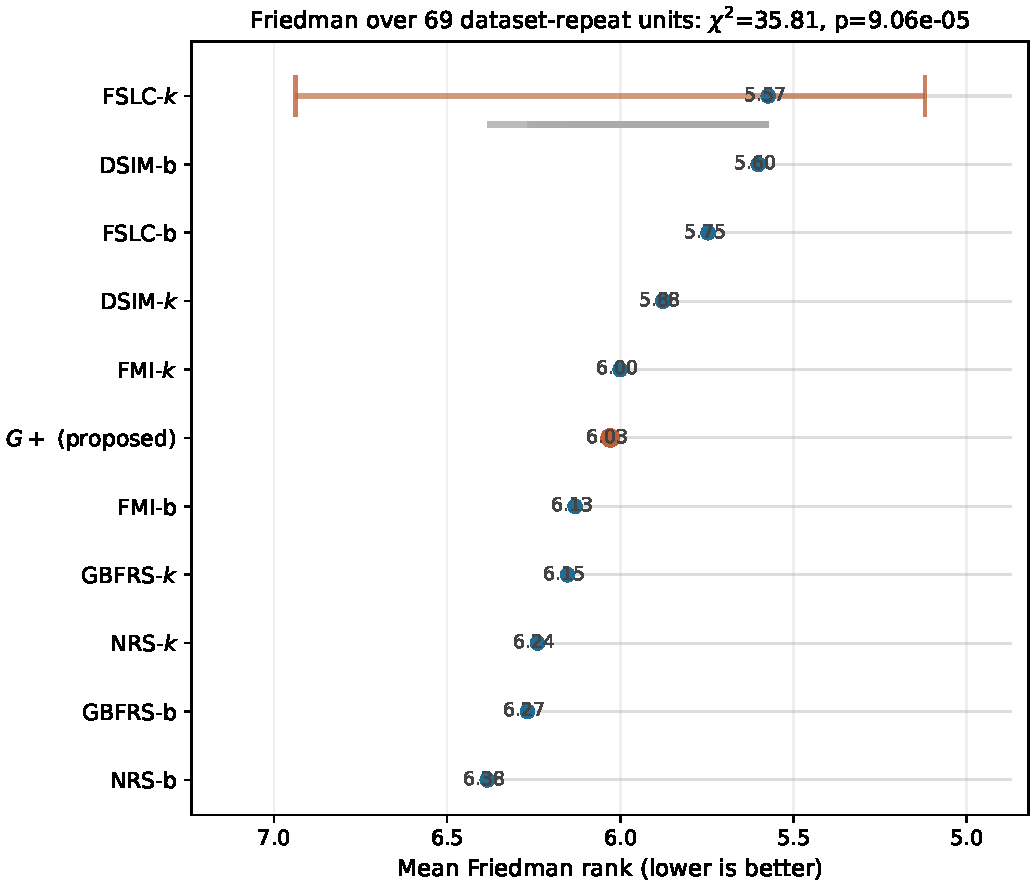
\includegraphics[width=\linewidth,height=.45\textheight,keepaspectratio]{paper_figures/expansion_cd.pdf}
	\caption{Mean Friedman ranks over the sixty-nine expansion dataset--repeat units (audit Brier; ties on guard-empty datasets receive average ranks), one row per method. The orange band is the Nemenyi critical difference (CD = 1.82) around $G+$; blue markers lie within it and are not statistically separated from $G+$.}
	\label{fig:expansion-cd}
\end{figure}


\subsection{Algorithmic Verification and Methodological Scope}
\label{subsec:logic-verification}

To confirm the operational integrity and implementation fidelity of the proposed optimization framework, we perform systematic verification across synthetic benchmark structures and delineate the methodological scope of the empirical evaluations.

\paragraph{Exact Search Verification on Synthetic Benchmark Topologies}
We benchmarked the exact branch-and-bound optimization implementation (Section~\ref{subsec:exact-search}) against exhaustive minimum-cost enumeration across $80$ synthetic non-monotone loss-dependency profiles ($m=6$ attributes). The algorithm achieved $100\%$ exact solution agreement across all evaluation scenarios. Specific stress-test configurations confirmed the algorithmic handling of critical boundary cases:
\begin{enumerate}[label=(\arabic*), leftmargin=*]
	\item \textbf{Sub-Floor Singletons:} Correct identification of highly predictive individual attributes situated below the historical dependency threshold;
	\item \textbf{Synergistic Feature Pairs:} Accurate traversal of multi-attribute interactions across non-monotonic loss plateaus via the signed predictive bridge;
	\item \textbf{Degenerate Zero-Cost Optima:} Provable convergence to the empty attribute set ($P^* = \varnothing$) when structural feature signals fail to surpass the uninformative baseline.
\end{enumerate}
These formal checks confirm that the branch pruning logic and feasibility enforcement operate in exact conformance with the theoretical minimum-cost formulation.

\paragraph{Methodological Scope and Evaluation Boundaries}
To maintain rigorous methodological transparency, we explicitly define the operational boundaries of the reported experiments:
\begin{enumerate}[label=(\arabic*), leftmargin=*]
	\item \textbf{Scoring Core Evaluation:} In Section~\ref{sec:paper-published}, competing methods are benchmarked by isolating their core representation scoring metrics within a unified, standardized evaluation pipeline. While this controls for extraneous algorithmic discrepancies (e.g., heterogeneous stopping criteria or auxiliary preprocessing), broader end-to-end pipeline comparisons under diverse downstream learners represent a valuable direction for future multi-center studies.
	\item \textbf{Scalability and Exact Optimality Gaps:} The branch-and-bound solver provides theoretical exactness for compact problem instances, but exhaustive exploration becomes computationally prohibitive on high-dimensional datasets. In large-scale real-world deployments, the guided heuristic search ($G/G+$) serves as an effective, polynomial-time surrogate, balancing feature acquisition costs against predictive loss feasibility.
\end{enumerate}
\section{Discussion}
\label{sec:discussion}

The proposed framework establishes a clear separation of concerns among its core components: local information weights quantify supervised distributional associations, granular dependency evaluates training representation coverage, and the inner-fold loss guard delineates a predictive feasibility boundary. A primary theoretical insight of this decoupling is that maximizing training-internal representation quality does not universally guarantee out-of-sample prediction preservation. By acknowledging non-monotone granular gains, the search mechanism naturally accommodates structural reformations in granular space without compromising exact cost-based branch pruning.

Our empirical findings provide critical insights into the operational trade-offs of cost-sensitive LDL reduction. Across twenty-five native benchmarks, the framework identifies highly informative attribute subsets at ultra-low acquisition costs compared to matched label-free baselines. Crucially, the multi-domain expansion reveals that the near-degenerate regime first observed on \emph{Yeast-cold} and \emph{Human Gene} is the dominant case rather than an exception: on twenty of the twenty-five benchmarks, the mean-distribution predictor itself achieves optimal audit performance under the Euclidean $k$-NN protocol. In such cases, returning an empty set at zero cost is not a predictive failure, but rather the theoretically correct and most cost-effective response. Furthermore, scenarios where nonempty subsets underperform the empty baseline (e.g., boundary cases under uninformative predictors) highlight the essential role of internal feasibility checks in preventing unnecessary feature acquisition. While granular guidance effectively navigates complex search spaces to discover non-dominated low-cost candidates, its performance gains interact with dataset geometry and cost distribution topologies.

To maintain methodological rigor, future confirmatory evaluations should preserve the frozen algorithmic structure while expanding the experimental scope across diverse multi-source cost scenarios and heterogeneous LDL predictors. In addition, assessing exact search methods on compact real-world instances will further illuminate the trade-offs between heuristic optimality gaps and computational overhead.

\section{Conclusion}
\label{sec:conclusion}

In this paper, we presented a novel cost-constrained attribute reduction framework tailored for Label Distribution Learning (LDL). By combining local distribution-information weighting with a source-dependent directed dissimilarity, our approach captures both supervised label associations and continuous geometric structures without forcing rigid metric symmetry. We established that distance monotonicity under fixed statistics does not automatically guarantee monotone granular dependency—a theoretical insight that motivates our non-monotone granular-ball representation. To address this, we cast attribute reduction as a minimum-acquisition-cost optimization task subject to an internal prediction-loss constraint, decoupling dynamic granular dependency guidance from predictive feasibility guarantees. 

Extensive experiments across twenty-five native LDL benchmarks demonstrate that the proposed framework cuts feature acquisition costs by over two orders of magnitude while strictly maintaining predictive feasibility. Benchmark comparisons against five published scoring cores spanning 2022--2025 confirm that our method avoids exorbitant acquisition expenses for equivalent or superior prediction loss. Crucially, our empirical analysis uncovers near-degenerate regimes where the zero-cost baseline is optimal, underscoring the necessity of evaluating internal feasibility rather than enforcing artificial "lossless" reduction; the guard ablation shows that guard-free selection actively wastes budget on these domains, and the predictor-sensitivity study shows the same guard certifying low-cost dominant subsets on revived domains once a suitable predictor is deployed, on six of nine such datasets outperforming both the zero-cost and full-cost references at $1$--$6\%$ of full-set cost.

Future research will extend this framework to online and streaming LDL scenarios, investigate adaptive prediction-loss bounds under multi-source cost heterogeneity, and explore exact constraint-solving techniques for large-scale real-world deployments.

\clearpage
\section*{Declarations}

\subsection*{Originality Statement}
This manuscript has not been published previously and is not under consideration for publication elsewhere. All authors have approved the manuscript and agree with its submission to Applied Soft Computing. All content is original; no substantial parts have been published or submitted to another journal, and all third-party material is properly cited.

\subsection*{Funding}
This work was supported by the National Natural Science Foundation of China (Grant No. 11971420).

\subsection*{Competing Interests}
The authors declare no financial or non-financial competing interests relevant to this work.

\subsection*{Ethics Approval}
This work is a secondary computational analysis of publicly available LDL benchmark datasets (e.g., Natural Scene, SBU-3DFE, the Yeast gene-expression series, SJAFFE, FG-Net, Movie, and Human Gene; the complete list with sources is given in Table~\ref{tab:datasets}). No experiments involving human participants or animals were performed by the authors, and no new participant data were collected. The original datasets were collected and released under the ethics approvals and consent procedures documented by their respective custodians and are distributed for research use.

\subsection*{Consent to Participate and Consent for Publication}
Not applicable. This study uses only publicly available benchmark datasets; no new participant data were collected by the authors. Consent for the original data collection and public release was obtained by the original data custodians.

\subsection*{Data Availability}
The label distribution learning datasets analysed in this study are publicly available from the official LDL-LDM and PyLDL repositories. Source URLs, repository commits, and file hashes are recorded in the dataset source manifests within the reproducibility archive. Reanalysis scripts and result files supporting the findings of this study are available in the accompanying reproducibility archive.

\subsection*{Code Availability}
The source code and frozen result files supporting the conclusions of this article are archived at \url{https://github.com/barbarossa-li/ldl-cost-sensitive-reduction} and will be made publicly available upon acceptance.

\subsection*{Author Contributions}
\textbf{Chaoyang Li}: Investigation, scoring execution, formal analysis, writing---original draft preparation. \textbf{Xiaohan Li}: Conceptualization, methodology,  visualization, validation, resources. \textbf{Zhaowen Li}: Data curation, supervision, project administration, writing---review and editing, funding acquisition.  All authors have read and approved the final version of the manuscript.

\subsection*{Use of Generative AI}
During the preparation of this work, the authors used generative AI tools solely for the purpose of English language editing and text polishing. Following the use of these tools, the authors reviewed and edited the content as needed and accept full responsibility for the final published content. No AI tools were used to generate research hypotheses, experimental results, or conclusions.

\bibliographystyle{elsarticle-num}
\bibliography{refs_updated}
\end{document}
